%
% File acl2020.tex
%
%% Based on the style files for ACL 2020, which were
%% Based on the style files for ACL 2018, NAACL 2018/19, which were
%% Based on the style files for ACL-2015, with some improvements
%%  taken from the NAACL-2016 style
%% Based on the style files for ACL-2014, which were, in turn,
%% based on ACL-2013, ACL-2012, ACL-2011, ACL-2010, ACL-IJCNLP-2009,
%% EACL-2009, IJCNLP-2008...
%% Based on the style files for EACL 2006 by 
%%e.agirre@ehu.es or Sergi.Balari@uab.es
%% and that of ACL 08 by Joakim Nivre and Noah Smith

\documentclass[11pt,a4paper]{article}
\usepackage[hyperref]{acl2020}
\usepackage{times}
\usepackage{latexsym}
\renewcommand{\UrlFont}{\ttfamily\small}
\usepackage{lipsum}
\usepackage{graphicx}
\usepackage{xcolor}
\usepackage{amsmath,amsthm,amssymb}
\usepackage{booktabs}
\usepackage[subtle]{savetrees}

\usepackage{tabularx}
\usepackage{multirow}
    \newcolumntype{L}{>{\raggedright\arraybackslash}X}

\usepackage{arydshln}

\setlength\dashlinedash{0.2pt}
\setlength\dashlinegap{1pt}
\setlength\arrayrulewidth{1.2pt}

% This is not strictly necessary, and may be commented out,
% but it will improve the layout of the manuscript,
% and will typically save some space.
\usepackage{microtype}

%\aclfinalcopy % Uncomment this line for the final submission
%\def\aclpaperid{***} %  Enter the acl Paper ID here

%\setlength\titlebox{5cm}
% You can expand the titlebox if you need extra space
% to show all the authors. Please do not make the titlebox
% smaller than 5cm (the original size); we will check this
% in the camera-ready version and ask you to change it back.

\newcommand\BibTeX{B\textsc{ib}\TeX}

%\title{Toward Long-Tailed Language Models\\ with Continuous-Output Prediction}
\title{If it's not the decoding maybe it is the approach:\\ How to overcome the long-tail problem in language model}

\author{Shiran Dudy\qquad Steven Bedrick\\
		Center for Spoken Language Understanding \\
	    Oregon Health \& Science University\\
	    3181 S.W. Sam Jackson Park Rd.\\
	    Portland, Oregon, USA\\
	    {\tt \{dudy,bedricks\}@ohsu.edu}}

\date{}

\begin{document}
\setlength{\abovedisplayskip}{0.5em}
\setlength{\belowdisplayskip}{0.5em}


\maketitle
\begin{abstract}
Neural language models typically employ a categorical approach to prediction and training, leading to well-known computational and numerical limitations. 
An under-explored alternative approach is to perform prediction directly against a continuous word embedding space. 
For large-vocabulary language models, this approach can not only result in smaller and simpler models but is shown here to reach low-frequency vocabulary words that are often ignored by the categorical model. Such words are essential, as they can contribute to personalization and user vocabulary adaptation.
In this work, we explore continuous-space language modeling in the context of a word prediction task over two different textual domains (newswire text and biomedical journal articles). 
We investigate both traditional and adversarial training approaches, and report results using several different embedding spaces and decoding mechanisms. 
We find that our continuous-prediction approach outperforms the standard categorical approach in terms of term diversity, in particular with rare words. 

\end{abstract}

\section{Introduction}\label{sec:intro}



 Neural approaches to language modeling have demonstrated substantial improvements in performance in recent years~\citep{melis2018on,merity2018regularizing}, and the latest techniques produce high-quality predictions across many benchmarks~\cite{peters2018deep,devlin2018bert}. % Bert, elmo
 Recently, we noticed that language generation suffers from a problem. The generated text is repetitive, dull, and generic. Various appraoches are aimed at tackling this issue in the form of decoding. Sampling, tenperature, nuleus, unlikelihood, bigger LMs, fine tuning LMs.
 The intuition of word pieces or BytePair made sense. refactoring the disrtibution across smaller vocab size. We would like to reframe the problem. This problem was already observed in other fields. We propose to look at it as the Long-Tail problem. Our task is based on directed prediciton, in other words we expect a specifc word to predicted as opposed to freely creating text. Therefore, our focus is not on generating surprizing text, rather predicting infrequent, yet learned text. We propose that while this is a different task the intuition behid surprisal is of similar nature of rare terms, both are unexpected given their context when employing current models. The ability to generate rare words types in language generation has been evaluated in the recent years...
 Given that similar architectures have been in use in domains like image and speech, employed for classiifcation, we have reasons to beliven that with current appraoches it still remains a challnage to retrieve diverse predictions as presented in typical human speech. This is our focus in the paper. 
% This performance comes at a price: most current SotA models employ deep architectures that are computationally complex and require a significant number of parameters to be learned. 
% According to~\citet{jozefowicz2016exploring} ``the best (language) models are the largest we were able to fit into a GPU memory'' suggesting that good model performance is conditioned on the access to heavy computational resources. 
% One major reason for this is that traditional approaches to language modeling (both neural and otherwise) treat the task as one of \textit{categorical} prediction: given some history of discrete symbols, each drawn from a finite set or vocabulary of size $V$, predict the next symbol in a sequence.\footnote{The symbols may be words, or sub-word units such as characters or other forms of glyph, depending on the level at which the model is operating.%(see section~\ref{subwords}).
% }
% % TBD

% In this work, we propose a simplified architecture and decoding strategy for training neural language models for use in explicit word prediction tasks, such as machine translation or predictive typing, in which the end goal is to identify target words.\footnote{As opposed to (e.g.) a representation learning application.} 
% Rather than performing a categorical selection from a fixed vocabulary of symbols, we predict a position in a continuous embedding space, and (if needed) decode from there into a discrete symbol. 
% In this, we follow the example of~\citet{kumar2018mises} and~\citet{li2019efficient}, who explored similar approaches as part of machine translation and representation learning systems, and instead apply it directly to the problem of word prediction in a typing scenario.

% Our proposed approach demonstrates enhanced performance when compared to a categorical baseline in prediction of low frequency words, often referred as the ``long-tail'' words of the vocabulary. In addition to having a smaller computational footprint and fewer parameters than the traditional categorical approach, our continuous approach opens the door to more flexible options for open-vocabulary and domain-adapted language modeling.

% This is particularly important in text entry scenarios, such as that found in mobile device keyboards, as well as in augmentative and alternative communication platforms for use by individuals with communication-related disabilities~\citep{Higginbotham:2012aa, Fager:2019aa, dudy2018compositional}.
% Such systems must continuously adapt to their users over time, and also frequently must accommodate novel and rare vocabulary items, depending on their users' needs. 
% This represents a major limitation for traditional categorical-prediction neural language models, as adapting the standard architecture to support entirely new vocabulary items requires structural changes to the output layer, which in turn requires the model to be re-trained.

% The text entry use case depends directly on word prediction, in which a language model is given some history of previously-selected tokens and must suggest a small set of likely continuations.
% This restriction implies that models used for text entry must be unidirectional, as ``future'' token information is not accessible to the model while the user is typing. 
% The text entry scenario also has implications for model evaluation and comparison.
% In this work, we focus on evaluating our language models with practically-motivated metrics which allow us to explore patterns that often are overlooked in conventional language model studies. 

% Predicting continuous vector representations holds promise particularly for overcoming non-stationary distributions as new vocabulary ``types'' are introduced, but also as underlying distribution for different terms may change over time. 
% This approach is not bounded to complexity issues resulted of vocabulary size ($|V|$) dependency as there is no need for a softmax layer. 
% Rather, the embedding dimensionality ($d$) determines the model's complexity, and is often orders of magnitude smaller than a typical vocabulary size, thereby reducing the model's footprint and training requirements. 

% This paper's contributions are as follows: (a) we experimentally investigate the performance characteristics of categorical and continuous approaches for language modeling, applied to a word prediction task, with a particular focus on infrequent words, on two distributionally different domains; (b) we introduce means to further augment the continuous approach by proposing a new decoding mechanism, and evaluate its use across different embedding spaces; (c) we propose a GAN-based architecture and compare it to a simple continuous architecture; and, (d) we provide evidence for the importance of taking word frequency into account when evaluating language model performance. 


\section{Related work}\label{work}

\textbf{Predictive Language Models}. While there exists a great deal of work regarding categorical-prediction language models, continuous-prediction is less well-studied. 
The closest and most relevant recent work is that of~\citet{kumar2018mises}, who also explored direct prediction of continuous word embeddings, albeit in the context of Neural Machine Translation. 
They proposed a new loss function for that purpose and demonstrated their model's feasibility over a large-vocabulary task.
\citeauthor{kumar2018mises}'s approach also demonstrated good performance at translating low-frequency source words into higher-frequency target language terms by leveraging properties of the target embedding space. 
Subsequent work by~\citet{li2019efficient} focused on improving training times for ELMo models by using continuous output layers, and stressed the resulting reduction in computational cost while maintaining on-par performance on standard evaluation tasks. 

Our work differs from this work on continuous-space language modeling in that we focus specifically on a word prediction task, rather than a MT or a contextual representation task.
%Another important difference is our work's 
Additionally, our primary focus is on accurately modeling rare vocabulary entries, as well as our investigation of different embedding spaces and their impacts.

\noindent
\textbf{Adversarial Language Model Training}. 
%Together with that, we explore the use of generative adversarial networks (GANs) to the problem of training our continuous-prediction language model and propose a new decoding mechanism over a simple nearest neighbor approach.
GANs are infrequently used in language modeling, and existing work has emphasized language generation~\citep{subramanian,press2017language}.
In part, this is due to a fundamental mismatch between the discrete, sequential, and variable nature of traditional language modeling and the more static, real-valued, continuous space in which GANs work. 
\citet{yu2017seqgan} proposed a method for integrating an RNN into the generator component of a GAN and solved certain issues relating to gradient updates, which led to a successful MT architecture by \citep{yang2017improving}.

Our model (see section~\ref{baseline}) follows the Conditional GAN architecture described by \citet{mirza2014conditional}, which provides the discriminator with jointly encoded representations of both genuine and false sequences. In our case, we have extended it to work with continuous-space word embeddings as output.

\noindent
\textbf{Rare Words}. Rare words are a persistent source of difficulty in neural approaches to NLP. 
In the context of NMT, \citet{sennrich2016neural} demonstrated that rare words were more optimally predicted by using subword units, and this has since become a common practice. 
However, recent work by~\citet{czarnowska2019don} has shown that subword units can cause other problems in morphologically rich languages, and found that systems struggled with achieving both semantic and morphological correctness.
This is particularly problematic in domains with high vocabulary diversity, such as biomedical literature.

Embedding spaces are another area of focus for rare words. \citet{pinter2017mimicking} devised an approach to adding high quality representation of rare terms to an embedding space by generating new items based on learning a word's embedding from its characters; its extension by~\citet{schick2019attentive} also employed the word's contexts. 
\citet{bojanowski2017enriching} also addressed rare words by extending a skipgram model to include subword units to improve the representation of rare terms.
%, and in~\citet{pilehvar2018card} with forming lists of rare word pairs for similarity evaluation of embeddings. 2 more papers that we have no room to add CHARAGRAM, Compositional-ly Derived Representations of Morphologically Complex Words in Distributional Semantics
Despite this research focus on the prediction and modeling of rare words, there is a noticeable lack of standard evaluation metrics and methods that focus specifically on rare-word performance.

 %there are two well known datasets of rare words stanford's RW (not cited) and CARD (cited)


\section{Methods}\label{data}

\subsection{Models \& Training}\label{baseline}

We developed three families of model\footnote{Code and pre-trained models are available at [URL MASKED].}. 
First, a simple implementation of a traditional categorical model (referred to as {\tt ctg}). 
Second, a continuous-prediction model, described below ({\tt c}). 
Third, a version of {\tt c} that was trained as a generative adversarial network ({\tt G}). We describe each model in detail below.

The categorical discriminative LSTM ({\tt ctg}) is based on the method of~\citet{sutskever2011generating}, using word embeddings as inputs, a unidirectional LSTM architecture with $200$ hidden units, and a standard cross-entropy loss function over a softmax output layer. 

For our continuous prediction model ({\tt c}), we use a similar input architecture, but with a fully-connected linear output layer instead of a sofmax layer. 
The output layer is of the same dimensionality as the input layer, and we train the model to attempt to directly predict the word embedding of the next timestep's word. 
As the loss function, we use the cosine distance between the predicted and target embeddings, using the ADAM optimizer.\footnote{During development, we also experimented with MSE and Max-Margin losses and found that cosine loss consistently performed best.}



\noindent
\textbf{GAN Architecture}
In addition to the basic continuous approach described above, we investigated a generative adversarial (GAN) approach. 
We employed the above-described continuous model as a Generator ({\tt G}), but in this case trained jointly with a Discriminator ({\tt D}) to provide stimuli for training the Generator. 
{\tt D} uses the same architecture as {\tt G}, but (following the approach of~\citet{mirza2014conditional}) during training is also provided with either a real or predicted (``fake'') embedding from {\tt G}. The discriminator compares its generated embedding with the provided sample, and must make a prediction about the sample's authenticity when compared to what it generated as described in equation~\ref{eq:disc_layer}.
\begin{equation} \label{eq:disc_layer}
%\vspace{-.075in}
D_t = \sigma \left ( (\hat{e}_D-e_{real,fake})^T \theta + b \right )
\end{equation}

Our final loss calculation (eq.~\ref{eq:gans}) closely follows the architecture used by~\citet{yang2017improving} and \citet{yu2017seqgan}, in that it conditions over a history of token vectors as input, but is different in its output, aiming to generate a vector representation (rather than a specific vocabulary item):
\begin{equation}\label{eq:gans}
  \begin{split}
\underset{G}{\text{min }} \underset{D}{\text{max }} L(D,G) = \\ 
\mathbb{E}_{w\sim{p_{data}(w)}}[\log D(w_t|w_{history})] + \\
\mathbb{E}_{\hat{w}\sim{p_{\hat{w}}(\hat{w})}}[\log (1-D(G(\hat{w_t}|w_{history})))]\\
\end{split}
\end{equation}
To the best of our knowledge, this is the first attempt to employ this type of model for vector embedding prediction. 
GANs are trained using a joint loss function; the Generator and Discriminator are trained under MSE loss as in equation~\ref{eq:gans}, and the Generator also uses the same cosine loss as is used in the \texttt{c} model as its embedding loss. 

\noindent
\textbf{Training Strategy:}
Given the major differences between the three models ({\tt ctg}, {\tt c}, and {\tt G}), we ensured a consistent comparison by holding constant the amount of data that was available during training to the model.
In our experiments below, each model was trained for a single epoch (i.e., one pass over each training example).
During training, we performed regular checkpointing, and after a full epoch of training, the checkpoint with the best performance on a validation data set was used as our final model. 

\subsection{Embeddings}\label{subsec:methods:embeddings}
In Section \ref{space} we evaluate the impact of the word embedding space on three different embedding spaces: Word2Vec~\citep{mikolov2013distributed}\footnote{Using the implementation by~\citet{rehurek_lrec}.}, GloVe~\citep{pennington2014glove}\footnote{~\url{https://github.com/stanfordnlp/GloVe}}, and FastText~\citep{bojanowski2017enriching}\footnote{~\url{https://github.com/facebookresearch/fastText}} ({\tt w2v}, {\tt ft}, {\tt glv} models), with dimensionality of $50$.\footnote{See Appendix \ref{embedding_apx} for a set of experiments with higher-dimensional embeddings.} 
We trained embedding models from scratch on the same data used to train the language models. 
In the experiments described in sections \ref{high_ana}, \ref{low_ana}, and \ref{decoding} we used word2vec as the embedding space. 

\subsection{Decoding}\label{subsec:dec}
The decoding process maps the embedding prediction to a point in the embedding space to associate the prediction with a word type. We investigated two different decoding strategies:

\noindent
\textbf{Simple Decoding:} Given a predicted word embedding, find the nearest-neighbor vocabulary entry in the pre-trained embedding space. To perform efficient nearest-neighbor search, we use random projections with the \texttt{Annoy} library~\citep{Bernhardsson:2018aa}.


\noindent
\textbf{Feature-Based Decoding:} To augment nearest-neighbor decoding, we propose to filter the candidate neighbors using additional features.
In this work, we focus on using part of speech (PoS) information to assist in decoding such that the prediction is formed by a list of nearest terms that are associated with the PoS tag for the target word, in a related manner to the procedure described by~\citet{czarnowska2019don}. 
For the purposes of validating this approach, we use a feature oracle to provide the PoS data for the experiments in this paper; in practice, of course, an additional prediction would be necessary. 
Section~\ref{decoding} provides additional discussion of this aspect of our approach.

\subsection{Experiments}

We experimentally evaluate our three architectures using an online word prediction task, in which the model is provided with a word history and is queried for the subsequent token. 
This is a common method for training and evaluating language models, but in our case, we are much more interested in concrete measures of performance (word prediction accuracy and diversity of predicted terms) than we are in more abstract measures (perplexity, etc.).
In our experiments, we investigate the effects of model dimensionality, training method (continuous vs GAN) and decoding strategy (with and without feature-based decoding) on word prediction performance. 
We perform these experiments over two corpora, with very different vocabulary distributions and counts.

\subsubsection{Datasets}
We performed experiments on two corpora: newswire text from the New York Times section of the Annotated English Gigaword corpus~\citep[LDC2018T20]{ferraro2018english}, and full-text biomedical journal articles from the open-access subset of PubMed Central~\citep{beck2010report} (PMC). The PMC corpus was part-of-speech tagged using ScispaCy~\citep[Version 0.2.2, model: \texttt{en\_core\_sci\_md}]{Neumann2019ScispaCyFA}. 
These two corpora differ not only in their content, but also in their vocabulary.
PMC contains a much larger variety of word types, and includes many more tokens from from low-frequency types (``long-tail types''), as shown in Figure~\ref{fig:nyt_pmc_distribution}.
%Table~\ref{types_tokens} describes the number of types and tokens for each experiment. 
%Figure~\ref{fig:nyt_pmc_distribution} shows a log-log scale of both datasets' distributions. 
%It describes how many types are found in different frequency bins, for instance in the frequency bin of $10^{0.5}-10^{1}$, the number of NYT types is about $310,000$, whereas for PMC it is more than twice as large at about $630,000$, emphasizing the longer tail phenomenon in PMC, presenting high number of low frequency words. 
%In contrast, there are more types in the NYT dataset from the high-frequency bins.
%Note that the PMC corpus exhibits a much greater relative diversity of types than the NYT corpus (i.e., it has a much ``longer tail'').
For the purposes of our experimental evaluation, we attempted to match the two corpora to have approximately the same vocabulary size, so as to ensure similar input dimensionality in the {\tt ctg}. As such, the NYT corpus is notably larger in terms of token count. 
There were $950$k types and $734$M tokens in the NYT corpus, and $860$k types and $458$M tokens in PMC.
\footnote{All vocabulary types observed fewer than four times in the training set were replaced with an \textit{unk} symbol, and numeric tokens were replaced with a class token.}

%APPX
%The results reported in this paper are were computed on the test set, though we note that no meaningful differences were exhibited in any of the dev/test pairs for any particular model; we used a 60/20/20 train/dev/test split.
% \begin{table}[h]
% \begin{center}
% \begin{tabular}{lrr}
% experiment &  num. types & num. tokens \\ \hline
% NYT & $950$k & $734$M  \\
% PMC & $860$k & $458$M  \\
% \end{tabular}
% \end{center}
% \vspace{-0.1in}
% \caption{\label{types_tokens} overall types and tokens}
% \vspace{-1.5em}
% \end{table}

\begin{figure}[h]
    \centering
    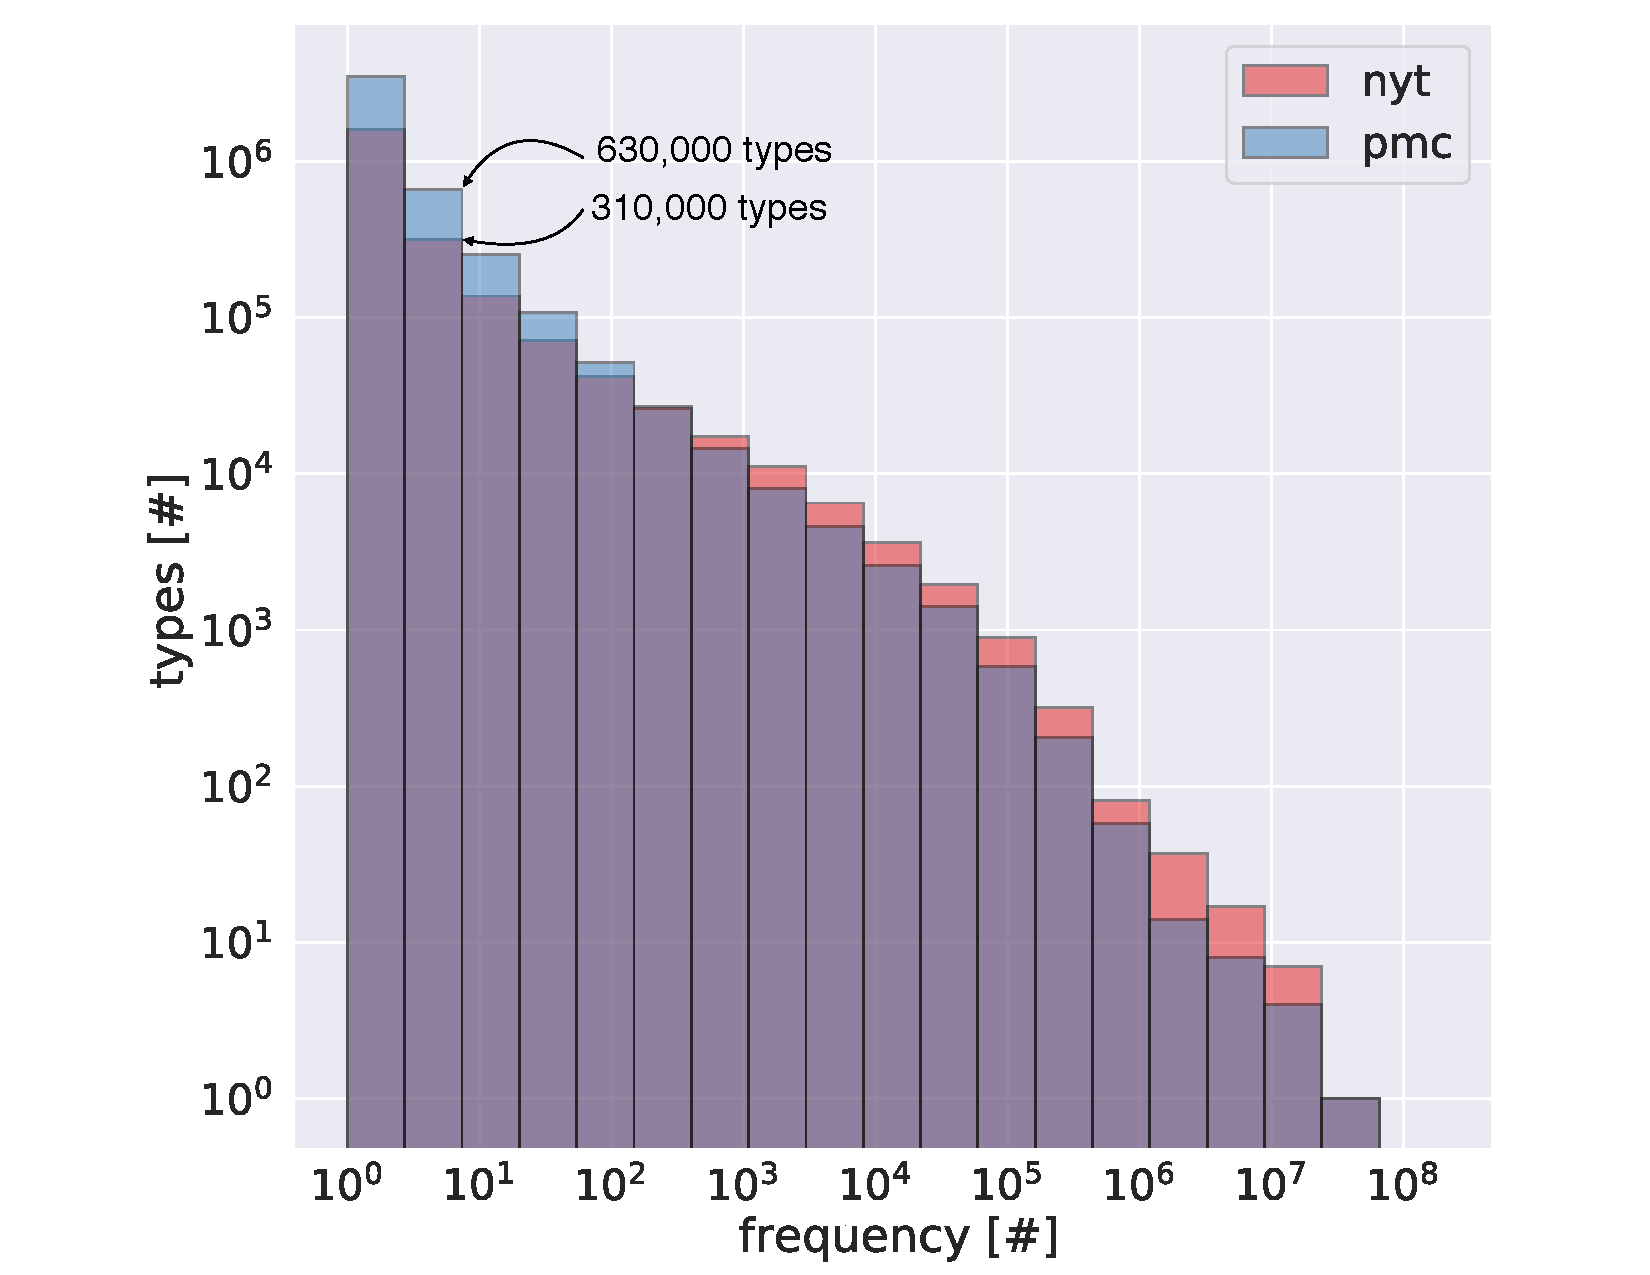
\includegraphics[width=0.4
    \textwidth]{fig/nyt_pmc_token_freq.pdf}
    %\vspace{-0.35in}
    \caption{token-type distribution}
    \vspace{-0.25in}
    \label{fig:nyt_pmc_distribution}
\end{figure}

\subsubsection{Metrics}

In our word prediction experiments, our key unit of evaluation was the prediction attempt: given a word history, was the model able to correctly predict the following token? 
We refer to this as a ``hit''. 
Because we are predicting in a continuous embedding space, it may be that various neighbors of the 1-best word are relevant or appropriate; furthermore, many real-world word prediction tasks involve presenting a user with a short set of candidates, so a near-miss may in practice still be a useful result.
As such, we also consider the neighborhood of the ten closest words to the predicted vector.
In addition to raw prediction performance, we are particularly interested in the \textit{diversity} of predicted types; a model that only ever predicted extremely common words could achieve a high accuracy score, but would be of no practical use. 
We used following metrics to evaluate our models: 

\begin{itemize}
 \setlength\itemsep{0.1em}
  \item $top_{1}(top_{10})$ - percentage of trials that constituted a  ``hit'' (i.e., target is within top 1/10 neighbor(s)) vs. a ``miss''
  \item $T_{1}(T_{10})$ - number of unique \textit{types} that the model correctly predicted (i.e., that appeared in at least one $top_{1/10}$ hit). 
  %In the correctly predicted sentence `it's a new dawn, it's a new day', since the system correctly predicted twice the category~\textit{new} this type is counted once. The final list is of a unique types that were correctly predicted at least once in the testset.
  \item $M$ - Mean Reciprocal Rank (MRR) of the targets w.r.t. their predictions (for ranks $<10$, MRR is 0).
\end{itemize} 

We compute these metrics over the predictions on the entire test set, and also break them out into vocabulary frequency bins. This allows us to investigate our models' performance on rare words.

\noindent
\textbf{A note on perplexity}: While perplexity is a traditional metric for evaluating language model performance, we do not use it in this set of experiments. 
This choice is driven first by the fact that our predictions, being in a continuous space, do not lend themselves naturally to perplexity calculation, and second, that our focus is on a practical application-oriented task (word prediction), where metrics such as $MRR$ are more closely linked to our outcome of interest. 
We would like to emphasize that the metrics proposed here reveal what perplexity may overlook, which is how well the model performs in practice, particularly regarding the variety of types the approach succeeded in predicting. 
%We will further be able to address later a finer granularity of predicted types namely whether the model was doing well only when the word is highly frequent, or attempted at predicting more rare ones.


\subsubsection{Baselines}

In our experiments, we compare our \texttt{c} and \texttt{G} models to our simple \texttt{ctg} model, as well as to two additional baseline models: \texttt{freq}, which consistently predicts the ten most common words in the test corpus, as well as \texttt{ugrm}, which randomly samples ten words from the test corpus's unigram distribution. 

The purpose of these frequency-based baselines is to account for the possibility of \textit{mode collapse}, a common failure mode in which a model learns to predict a small number of frequently-observed values.\footnote{GANs are notoriously prone to mode collapse.} 
We were particularly concerned about this failure mode given the heavily-skewed distribution of words in a linguistic corpus, and the fact that the distributional properties of word embedding spaces tends to be affected heavily by word frequency~\citep{Gong2018aa}. We therefore, devised the \texttt{freq} and \texttt{ugrm} baselines in order to simulate models suffering mode collapse.

%The purpose of the $top10$ baseline is to simulate a model that  how well a model can do simply by guessing  very frequent terms. 
%This models a scenario in which a language model memorized  very prominent types and experiences an optimal mode collapse w.r.t hits.
%The unigram model (ungrm) is guessing words based on sampling from the training set unigram distribution. The stratified random predictions provide a lower bound for performance rates in a non-learning enviroment that is based on the datsset distribution.

\section{Results}\label{sec:results}


\subsection{High Level Analysis}\label{high_ana}
\begin{table}[h]
\begin{center}
\begin{tabular}{lrrr}
model &  $top_{1}$ $(top_{10})$ & $T_{1}$ $(T_{10})$ & $M$ \\ \hline
\texttt{freq} & $00.89$ $(23.39)$ & $1$ $(10)$  &  $0.04$\\
\texttt{ugrm} & $00.71$ $(08.46)$ & $2,190$ $(5,592)$ & $0.02$ \\
\addlinespace[1ex]

{\tt mle}$_{50}$ & $19.19$ $(46.02)$ & $3,982$ $(7,559)$ & $0.27$  \\
%{\tt wpe}$_{50}$ & $22.79$ $(45.20)$ & $3,451$ $(7,607)$ & $0.35$  \\
{\tt wpe}$_{50,nyt}$ & $28.28$ $(52.61)$ & $4,037$ $(7,630)$ & $1.37$ \\

{\tt UL}$_{50}$ & $17.50$ $(39.99)$ & $4,523$ $(8,782)$ & $0.24$ \\
{\tt c}$_{50}$ & $17.31$ $(28.70)$ & $8,917$ $(22,509)$&  $0.21$  \\
{\tt G}$_{50}$ & $16.46$ $(27.45)$ & $11,534$ $(27,921)$ & $0.20$   \\
\addlinespace[1ex]

{\tt mle}$_{200}$ & $21.21$ $(47.87)$ & $4,163$ $(7,683)$ & $0.29$ \\
%{\tt wpe}$_{200}$ & $23.49$ $(46.27)$ & $3,959$ $(8540)$ & $0.36$ \\
{\tt wpe}$_{200,nyt}$ & $29.04$ $(53.51)$ & $4,225$ $(7,687)$ & $1.37$ \\
{\tt UL}$_{200}$ & $18.33$ $(41.24)$ & $5,596$ $(10,352)$ & $0.25$ \\
{\tt c}$_{200}$ & $18.94$ $(30.90)$ & $4,335$ $(13,087)$ & $0.23$  \\
{\tt G}$_{200}$ & $18.15$ $(29.15)$ &  $6,194$ $(17,905)$ & $0.22$  \\ 
\end{tabular}
\end{center}
\vspace{-0.1in}
\caption{\label{nyt} Experimental results on NYT corpus}
\vspace{-0.1in}
\end{table}

Table~\ref{nyt} presents the results of our various models ({\tt ctg}, \texttt{c}, and \texttt{G}) when evaluated against a newswire corpus. 
The \texttt{freq} model shows that simply picking the most frequent word achieves a $top_{1}$ hit rate of $0.89\%$, and the ten most frequent words hit $23.39\%$ of the time. 
This shows that by predicting a very small number of distinct types, a model can easily get relatively a high hit rate. 
The \texttt{ugrm} model correctly predicts $2,190$ types, giving a reasonable estimate of what a chance model might achieve in terms of type diversity, but reaches a much lower hit rate than the \texttt{freq} baseline. 


The first triple of space dimensionality $50$ in Table~\ref{nyt}, of models ({\tt ctg}$_{50}$, {\tt c}$_{50}$, and {\tt G}$_{50}$) demonstrates an interesting tradeoff.
While the $top_{1}$ for the categorical baseline, {\tt ctg}, performed more optimally than the categorical models, the continuous approaches outperformed the categorical model in terms of $T_{1}$, and successfully predicted more than twice of the distinct types that {\tt ctg} was able to predict (the effect was even more pronounced in terms of $T_{10}$).
Increasing the embedding dimensionality to $200$ in Table~\ref{nyt}, the continuous approaches ({\tt c}$_{200}$, and {\tt G}$_{200}$) again reached a lower absolute hit rates, but maintained their advantage in type diversity. 
%The simple categorical prediction model ({\tt cg})  unsurprisingly improves over the \texttt{ugrm} and \texttt{freq} baselines in terms of prediction accuracy, and correctly predicts twice as many types ($T_1$) as the \texttt{ugrm} baseline: $3,982$ vs $2,190$. 


\begin{table}[h]
\begin{center}
\begin{tabular}{lrrr}
model &  $top_{1}$ $(top_{10})$ & $T_{1}$ $(T_{10})$ & $M$ \\ \hline
\texttt{freq} & $00.89$ $(25.53)$ & $1$ $(10)$ & $0.05$ \\
\texttt{ugrm} & $00.76$ $(09.03)$  & $1,790$ $(4,619)$ & $0.02$\\
\addlinespace[1ex]

{\tt mle}$_{50}$ & $22.12$ $(48.02)$  & $4,764$ $(9,020)$ & $0.30$\\
%{\tt wpe}$_{50}$ & $19.04$ $(35.62)$ & $2,473(10,728)$ & $0.35$  \\
{\tt wpe}$_{50,pb}$ & $27.29$ $(50.23)$ & $3,020$ $(6,849)$ & $1.27$ \\
{\tt UL}$_{50}$ & $17.52$ $(39.69)$ & $4,780$ $(9,657)$ & $0.24$  \\
{\tt c}$_{50}$ & $19.89$ $(32.04)$  & $11,947$ $(34,641)$ & $0.24$ \\
{\tt G}$_{50}$ & $19.04$ $(30.41)$  & $18,040$ $(47,550)$  & $0.23$\\
\addlinespace[1ex]

{\tt mle}$_{200}$ & $22.92$ $(48.47)$ & $3,678$ $(7,006)$ & $0.31$ \\
%{\tt wpe}$_{200}$ & $19.46$ $(36.26)$ & $2,620$ $(11,977)$ & $0.36$  \\
{\tt wpe}$_{200,pb}$ & $27.85$ $(50.94)$ & $3,182$ $(7,389)$ & $1.28$ \\
{\tt UL}$_{200}$ & $18.80$ $(41.13)$ & $5,888$ $(10,785)$ & $0.25$ \\
{\tt c}$_{200}$ & $17.06$ $(30.88)$ & $6,083$ $(18,533)$ & $0.21$  \\
{\tt G}$_{200}$ & $20.67$ $(32.96)$  & $9,411$ $(28,164)$ & $0.24$\\ 

\end{tabular}
\end{center}
\vspace{-0.1in}
\caption{\label{pb} Experimental results on large PMC corpus}
\vspace{-0.1in}
\end{table}

Table~\ref{pb} presents similar pattern in baselines performance to Table~\ref{nyt} w.r.t. to PMC dataset. This Table shows stronger trends for the non-baseline approaches. According to Table~\ref{pb} in the first triples of dimensionality $50$ while the continuous approaches are two points below in $top_{1}$, the type diversity of $T_{1}$ of {\tt c}$_{50}$, and {\tt G}$_{50}$, is about three-folds, and four-folds w.r.t. {\tt ctg}. Increasing dimensionality, to $200$, produced ambivalent affects on the hit rate of the continuous approaches, and decreased the number of types, yet they were still more than $1.5$, $2.5$ for {\tt c}$_{200}$, and {\tt G}$_{200}$. In the PMC experiment increasing to $200$ dims contributed to higher hit rate for {\tt ctg}$_{200}$, but it reduced the number of types, {\tt ctg}$_{200}$ in NYT relatively maintained a similar number of types. Overall across domains, while hit rates for the {\tt ctg} approach are higher, the continuous models often predict correctly many more types, learning more patterns that are unique to the particular domain at hand. Finally, comparing {\tt G} to {\tt c} in Tables~\ref{nyt},~\ref{pb}, on both datasets NYT and PMC, we find that each of the approaches stands out for different reasons. {\tt G} tends to be more rich in types, while {\tt c} demonstrates higher hit rates reflecting the bias-variance tradeoff. Overall dimensionality of $50$ is more preferable for the continuous approach in terms of type diversity. 





% The continuous prediction models are presented in Table~\ref{nyt} below {\tt ctg}, with a naming pattern of [model type][dimensionality][decoding] ($p$ indicating the use of part-of-speech feature decoding). 
% When compared to the {\tt ctg} case, the continuous models achieve comparable $top_1$ hit rates (though suffer somewhat in $top_{10}$). 
% However, they consistently produce a much higher number of correctly-predicted types, with $T_{1}$ scores ranging between 1.5 to three times the number of types of {\tt ctg}, and with an even greater improvement in $T_{10}$ (2-4 fold increase over {\tt ctg}).

\subsection{Long-Tail Analysis}\label{low_ana}

Recall that we have a particular interest in our models' performance at predicting rare words, and want our continuous models to learn to predict items in both frequent and rare neighborhoods in the embedding space. 
We, therefore, performed a stratified analysis by target word frequency, to assess whether our models' behavior differed in rare vs. common words.
%Going deeper, we decided to find out what types the different models predict, we divided the types by their frequency observed in the train set (while the results are on the test set). Ideally, the models learn to predict different frequency types, in particular the continuous models would produce embedding estimations of that are point to various locations in the space, demonstrating flexibility and potentially a wide range of pattern learning. Conversely, if the predictions are centered in the mean of the embedding space (where the majority of frequent words is) it is less likely to reach low frequency terms as they tend to be positioned in the `suburb' to `rural' areas of the space.

\begin{figure}[h]
    \centering
    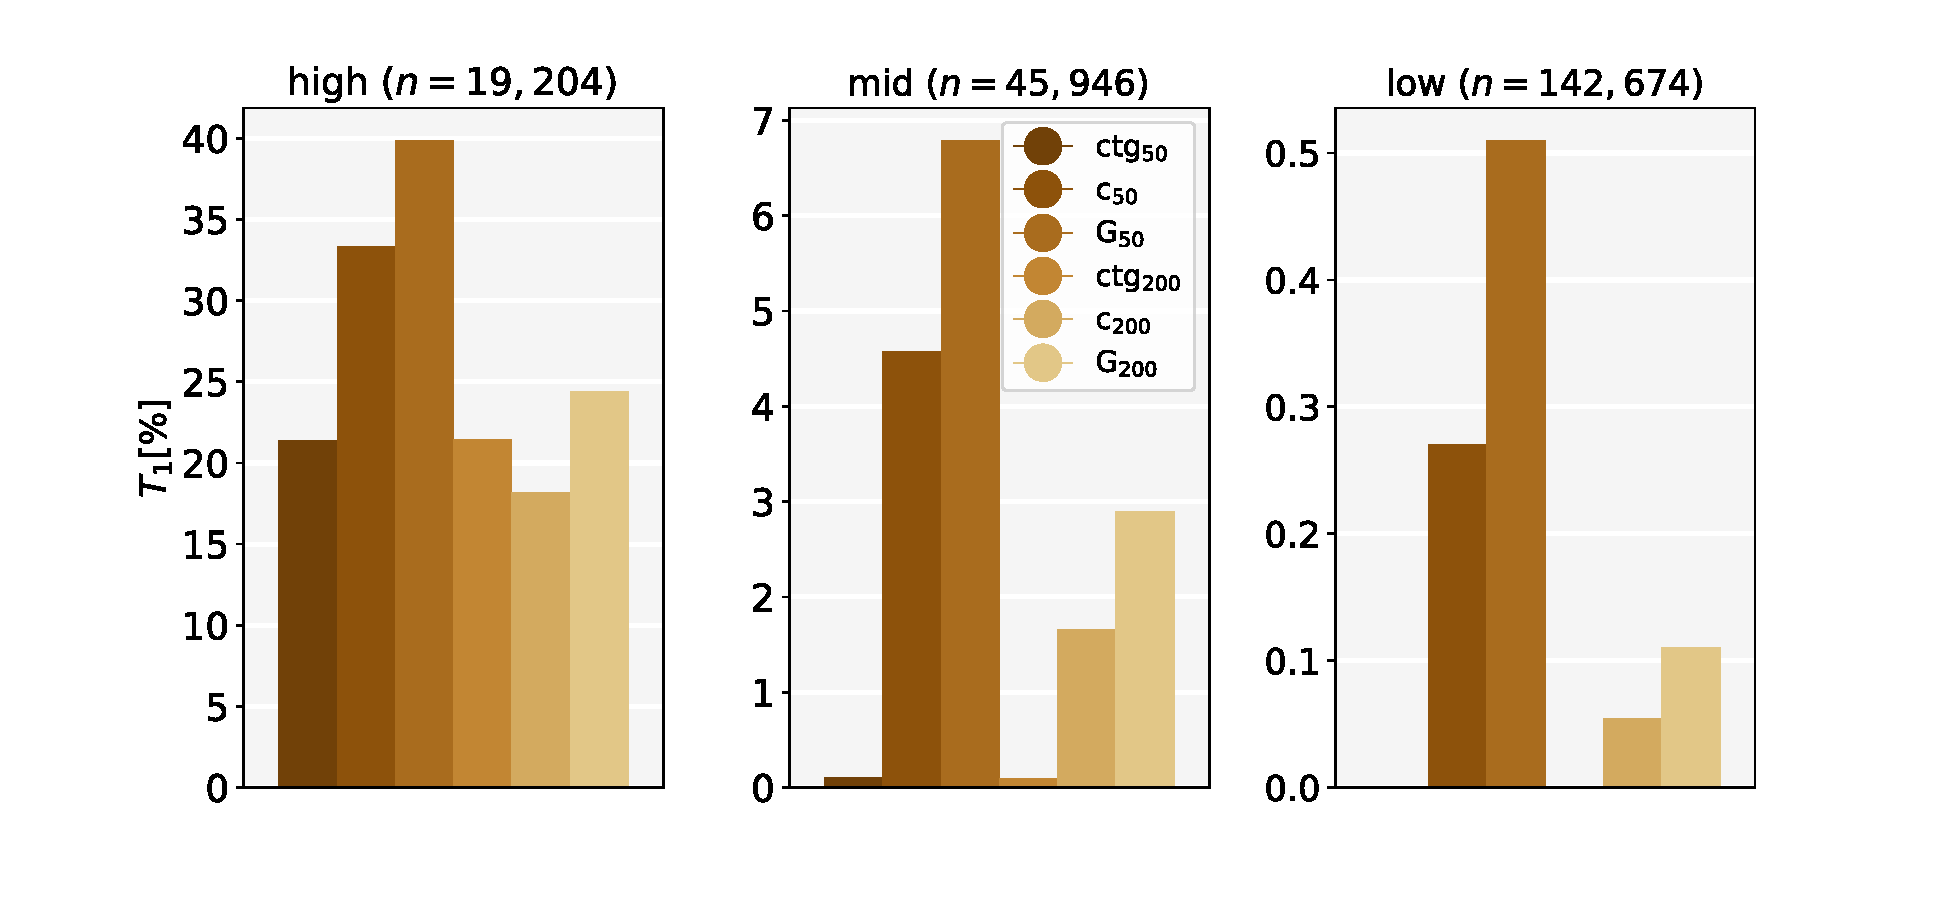
\includegraphics[width=0.47
    \textwidth]{fig/types_coverage_ny200.pdf}
    %\vspace{-0.35in}
    \caption{NYT \textit{type} coverage by training frequency bin. $n$: number of items in each bin; y-axes are percentages over $n$ (note different scales).}
    \vspace{-0.15in}
    \label{fig:type_coverage_ny}
\end{figure}


Figure~\ref{fig:type_coverage_ny} presents type coverage, for the NYT experiment, in three frequency bins: \textit{high}, \textit{mid}, and \textit{low}, for $x\in[10^3,\inf)$, $x\in[10^2,10^3)$, $x\in[10^1,10^2)$ where $x$ is each target type's frequency. 
We observe that the type coverage patterns of the models varies greatly across frequency bin.
In the high-frequency bin, the type coverage for {\tt ctg} is about $20\%$ for both $50$, $200$ dimensions (of total of $n=19,204$ types). 
The continuous approaches were more diverse than the categorical with $7,700$, $6,400$, $4,100$ types {\tt G}$_{50}$, {\tt c}$_{50}$, {\tt ctg}$_{50}$, whereas for $200$ dim, we observed no meaningful differences. 
For the mid- and low-freq bins, the continuous approaches clearly outperform their respective {\tt ctg} model. 
In the mid bin the {\tt ctg}$_{50}$ model was predicting as low as $55$ types, whereas {\tt c}$_{50}$, {\tt G}$_{50}$ demonstrated prediction of $2,100$, $3,100$ types respectively. 
Similarly, $40$, $760$, $1,300$, were correctly predicted types for {\tt ctg}$_{200}$, {\tt c}$_{200}$, {\tt G}$_{200}$. 
Among low-frequency types, there were no types predicted for any of the {\tt ctg} models, where $729$, $386$, $256$, and $78$ types were found in {\tt G}$_{50}$, {\tt c}$_{50}$, {\tt G}$_{200}$, {\tt c}$_{200}$ respectively.


% while most continuous models,  lower bound for any of the continuous models is at $30\%$. 
% In contrast, in the mid-frequency bin, the \texttt{cg} model achieves very little coverage, while the worst-performing continuous model reaches about $7\%$. 
% Among low-frequency types, the {\tt cg} was not able to make any correct predictions, whereas the continuous models were able to predict some types correctly. 
% While small in relative terms, this still resulted in anywhere from $1,800$ correctly-predicted types, to more than $3,600$ with $G_{50,p}$.

\begin{figure}[h]
    \centering
    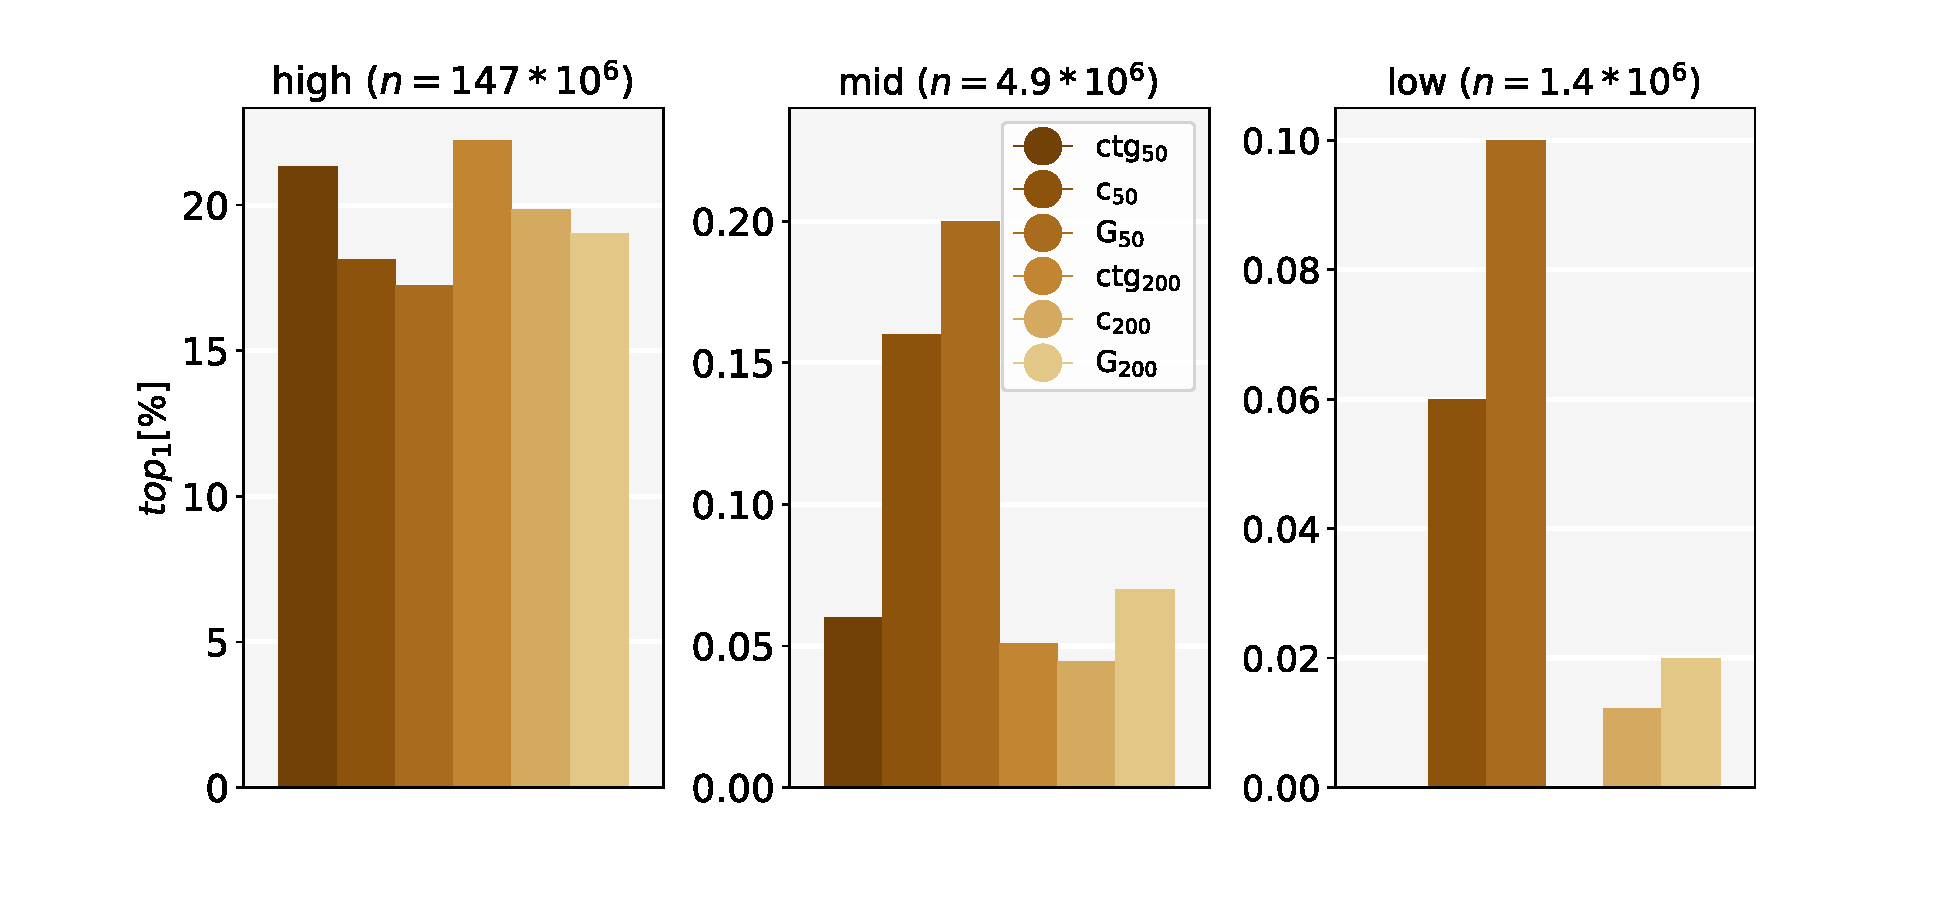
\includegraphics[width=0.47
    \textwidth]{fig/tokens_coverage_ny200.pdf}
    %\vspace{-0.35in}
    \caption{NYT \textit{token} coverage by training frequency bin. $n$: number of items in each bin; y-axes are percentages over $n$ (note different scales).}
    \vspace{-0.15in}
    \label{fig:token_coverage_ny}
\end{figure}

In addition to type coverage, we also performed a stratified analysis of \textit{token} coverage in Figure~\ref{fig:token_coverage_ny}. 
As before, we see a major difference across frequency bins, with all models performing substantially better on high-frequency terms, but with the traditional categorical approach struggling to make correct predictions on mid-frequency terms, and completely failing on low-frequency terms. 
We note that the mid-freq bin dim of $200$ was not so different among the three models. 
Our continuous models were able to correctly predict mid- and low-frequency terms often more times than their categorical counterpart.

\begin{figure}[h]
    \centering
    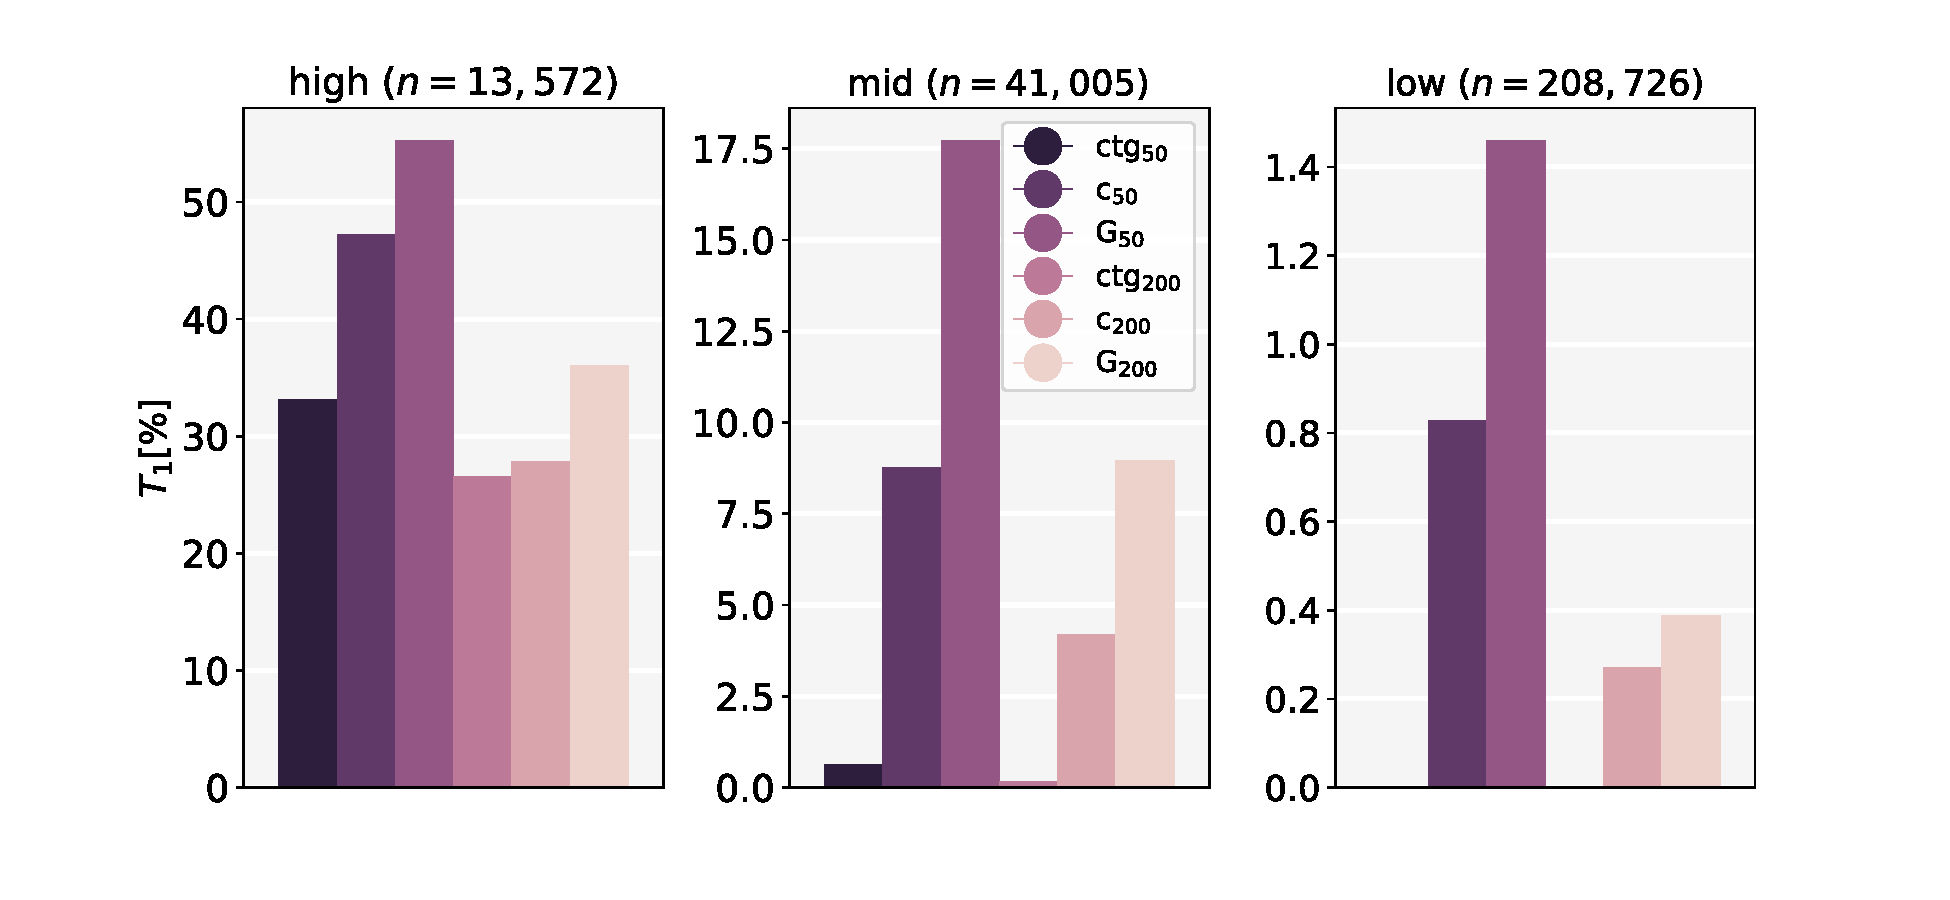
\includegraphics[width=0.47
    \textwidth]{fig/types_coverage_pb200.pdf}
    %\vspace{-0.35in}
    \caption{PMC \textit{type} coverage by training frequency bin. $n$: number of items in each bin; y-axes are percentages over $n$ (note different scales).}
    \vspace{-0.15in}
    \label{fig:type_coverage_pb}
\end{figure}


We applied the same analysis to the our results on the PMC dataset, which exhibited very different patterns of type distribution, as shown in Figure~\ref{fig:nyt_pmc_distribution}. 
Figure~\ref{fig:type_coverage_pb} demonstrates the type coverage of PMC across frequency bins. Here too, the differences are more pronounced in dim of $50$. 
Yet, for the majority of bins, the continuous approaches predicted more types, outperforming the {\tt ctg} models. 
In the mid bin types were of $7,200$, $3,600$, and $265$, for {\tt G}$_{50}$, {\tt c}$_{50}$, {\tt ctg}$_{50}$, and $3,700$, $1,700$, and $68$, for {\tt G}$_{200}$, {\tt c}$_{200}$, {\tt ctg}$_{200}$. 
Again, both {\tt ctg} models were unable to predict any types at all in the low bin, and $3,000$, $1,700$, $810$, and $565$ types were found in {\tt G}$_{50}$, {\tt c}$_{50}$, {\tt G}$_{200}$, {\tt c}$_{200}$ respectively. 

\begin{figure}[h]
    \centering
    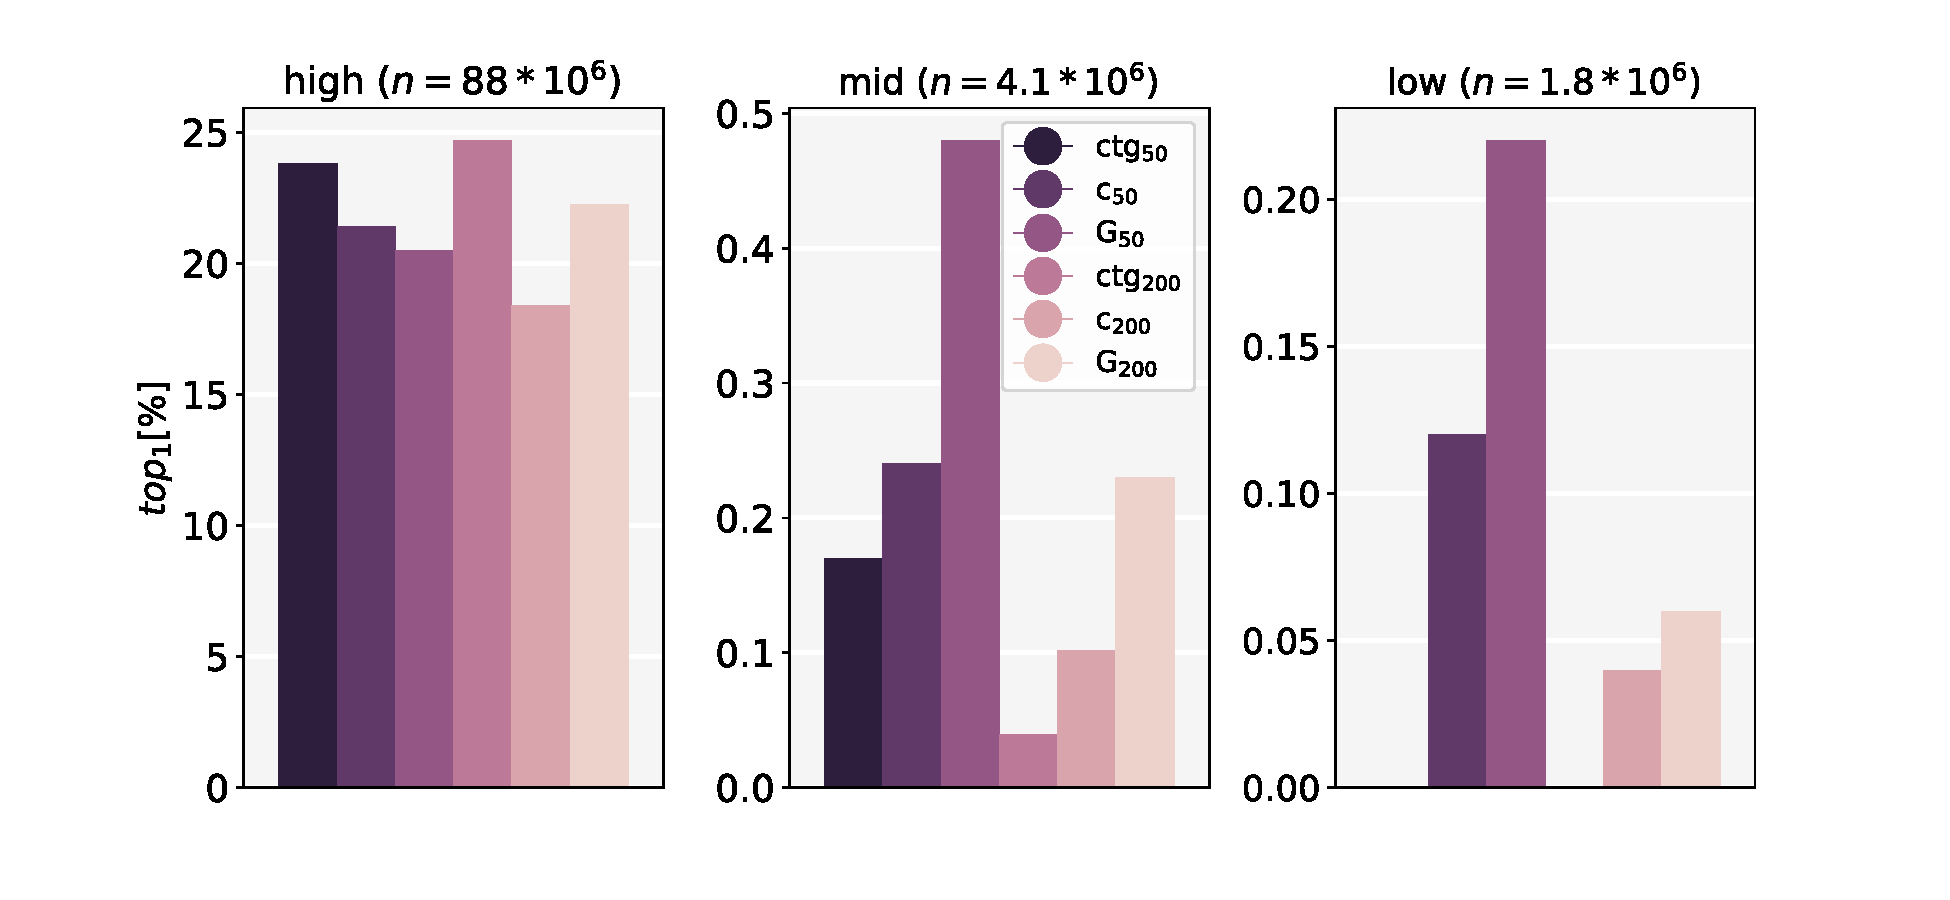
\includegraphics[width=0.47
    \textwidth]{fig/tokens_coverage_pb200.pdf}
    %\vspace{-0.35in}
    \caption{PMC \textit{token} coverage by training frequency bin. $n$: number of items in each bin; y-axes are percentages over $n$ (note different scales).}
    \vspace{-0.15in}
    \label{fig:token_coverage_pb}
\end{figure}

Figure~\ref{fig:token_coverage_pb} illustrates similar patterns to Figure~\ref{fig:token_coverage_ny}, but the richness in types for the continuous approaches in mid- and low-frequency bins is even greater.

This analysis shows that in longer-tail areas across domains, and longer tail domains, the continuous models are much stronger in terms of types diversity. 
We verified that the {\tt ctg} models' frequency-binned performance was significantly different from that of the continuous approaches statistically in Appendix~\ref{stat}. 
Additionally, see Appendix~\ref{qualit} for example word predictions from our various models across vocabulary frequency bins.  

%Before we continue to explore other facets of the continuous model, we would like to try out a different dataset, a corpus of academically written biomedical text. 

% \subsection{PubMed Central Experiment}\label{pb_sec}
% Text derived from biomedical literature typically has a very different term distribution than is found in typical newswire text, with a larger number of rare words (see Figure~\ref{fig:nyt_pmc_distribution}). 
% This is due to the presence of domain-specific terminology and jargon,  as well as the large variety of topics. 
% Language models trained on such text must therefore learn to model a much longer-tailed distribution of types.

% Table~\ref{pb_base} illustrates the results of our various models when trained and evaluated on this different corpus, in the same manner as described in the previous section.  
% Essentially, this set of experiments reveals similar patterns to those seen in the NYT experiment:  the various continuous-space approaches were generally comparable to the categorical baseline in terms of $top_{1}$, but outperformed the baseline in terms of type diversity ($T_{1/10}$). 
% This tendency was notably stronger in the PMC experiments. For $T_{1}$, the continuous approaches vary between twice to almost five times more than the number of types in the {\tt ctg}  approach (and between three to six times in $T_{10}$).  

% For both sets of experiments, when comparing the continuous models to one another, we see that {\tt G} was always more diverse than {\tt c}, while the {\tt c} had a slightly higher hit rate. 
% This suggests that the GAN training approach is helping the model learn to predict a broader range of vocabulary items.

% \begin{table}[h]
% \begin{center}
% \begin{tabular}{lrrr}
% model &  $top_{1}$ $(top_{10})$ & $T_{1}$ $(T_{10})$ & $M$ \\ \hline
% \texttt{freq} & $00.89$ $(25.53)$ & $1$ $(10)$ & $0.05$ \\
% \texttt{ugrm} & $00.76$ $(09.03)$  & $1,790$ $(4,619)$ & $0.02$\\
% \addlinespace[1ex]

% {\tt cg}$_{50}$ & $22.12$ $(48.02)$  & $4,764$ $(9,020)$ & $0.30$\\
% {\tt c}$_{50}$ & $19.89$ $(32.04)$  & $11,947$ $(34,641)$ & $0.24$ \\
% {\tt G}$_{50}$ & $19.04$ $(30.41)$  & $18,040$ $(47,550)$  & $0.23$\\
% \addlinespace[1ex]

% {\tt cg}$_{200}$ & $22.92$ $(48.47)$ & $3,678$ $(7,006)$ & $0.31$ \\
% {\tt c}$_{200}$ & $17.06$ $(30.88)$ & $6,083$ $(18,533)$ & $0.21$  \\
% {\tt G}$_{200}$ & $20.67$ $(32.96)$  & $9,411$ $(28,164)$ & $0.24$\\

% \end{tabular}
% \end{center}
% \vspace{-0.1in}
% \caption{\label{pb_base} Experimental results on large PMC corpus}
% \vspace{-0.1in}
% \end{table}

% Figures~\ref{fig:type_coverage_pb} and \ref{fig:token_coverage_pb} illustrate the results of our frequency stratification analysis on the PMC corpus, and tell a similar story as their NYT counterparts.
% The continuous models consistently outperform the categorical baseline in terms of type diversity ($T_1$), and on mid- and low-frequency words outperform the categorical baseline on token prediction accuracy ($top_1$). 

%Notably, on the PMC corpus, with its more diverse vocabulary, this performance gap between the categorical approach and the continuous approaches is greater than on the newswire text. 


% \begin{figure}[h]
%     \centering
%     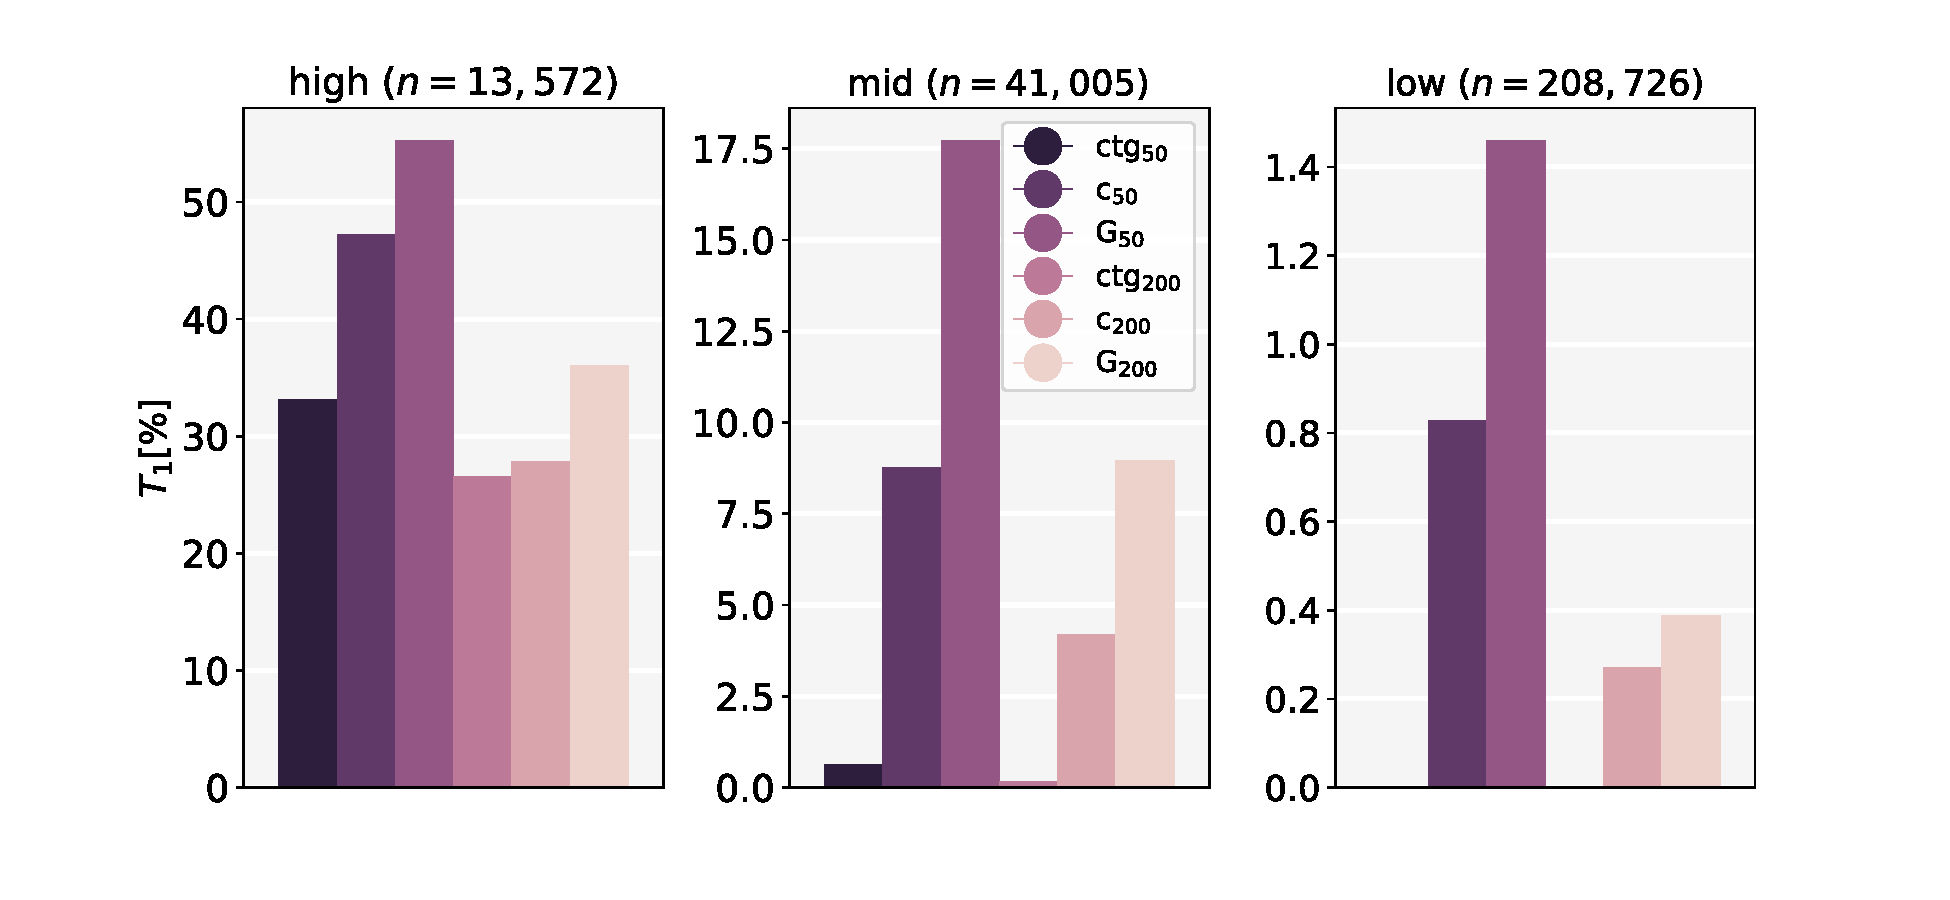
\includegraphics[width=0.47
%     \textwidth]{fig/types_coverage_pb200.pdf}
%     %\vspace{-0.35in}
%     \caption{PMC \textit{type} coverage by training frequency bin. $n$: number of items in each bin; y-axes are percentages over $n$ (note different scales).}
%     \vspace{-0.25in}
%     \label{fig:type_coverage_pb}
% \end{figure}

 

% \begin{figure}[h]
%     \centering
%     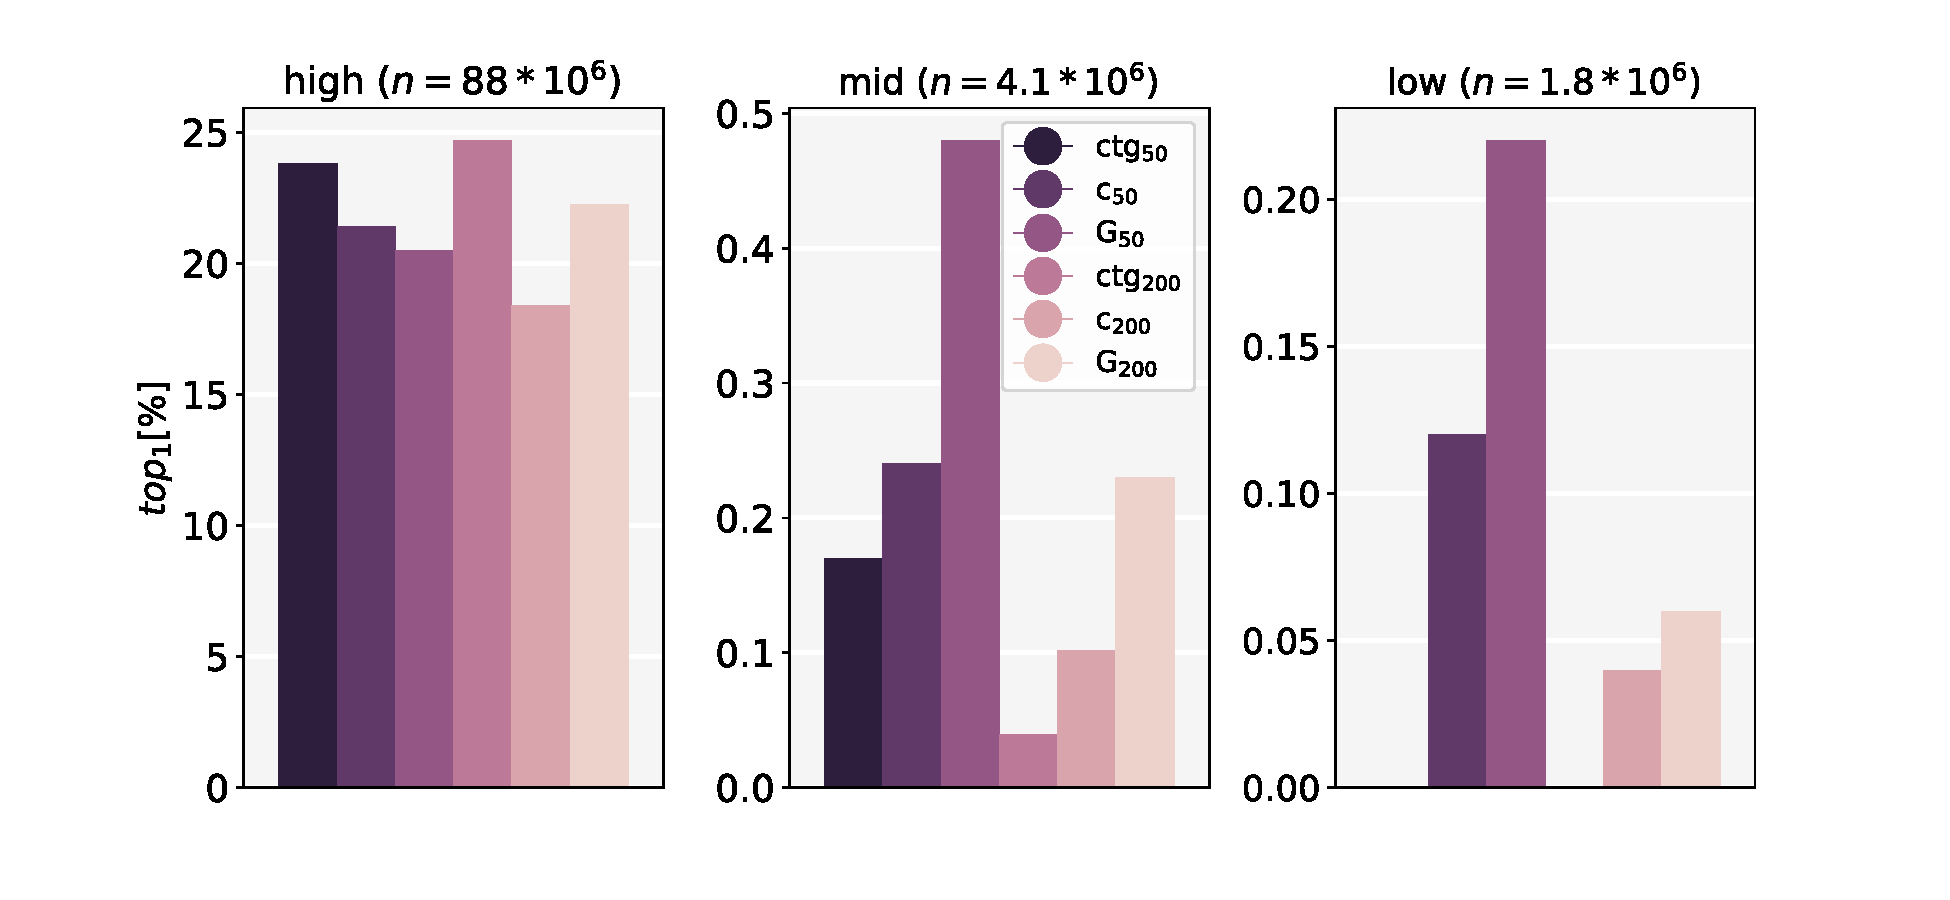
\includegraphics[width=0.47
%     \textwidth]{fig/tokens_coverage_pb200.pdf}
%     %\vspace{-0.35in}
%     \caption{PMC \textit{token} coverage by training frequency bin. $n$: number of items in each bin; y-axes are percentages over $n$ (note different scales).}
%     \vspace{-0.25in}
%     \label{fig:token_coverage_pb}
% \end{figure}

\subsection{Feature-Based Decoding}\label{decoding}

In the previous sections we showed that the continuous approaches, on both NYT and PMC datasets, produced models that were overall more diverse in their predictions than the categorical-based approach. 
We now propose a way to improve the hit rates of these approaches.  
Following the lead of~\cite{czarnowska2019don}, who focused on syntax prediction by fixing LM semantics, we fix/simulate the process of predicting PoS tags and focus on the semantic aspect of word prediction as described in.
Given that the embedding space these models learn is organized by semantic relations, e.g. words sharing similar context are likely to be found closer
we were curious whether adding \textit{syntactic} information could enhance the underlying results. 
For the purposes of this evaluation, we employed Feature-Based as decoding described in Section~\ref{subsec:dec} using  oracle PoS tags.~\footnote{See Appendix~\ref{simulation} for details on how we produced the oracles for our experiments}.
Note that this approach is highly flexible, as almost any feature (or combination of features) may be used to assist the model in decoding.
Given that, choosing \textit{which} feature(s) to use becomes an important question. If we had instead been using a word embedding space directly informed by syntax~\citep{levy2014dependency} or frequency~\citep{Gong2018aa}, a different choice of feature may work better. 
We also note that, in reality, PoS information is not generally available \textit{a priori} at inference time.
We justify our use of an oracle in this paper's experiments as follows: PoS prediction in English is a much more highly-constrained problem than full word prediction, and can be done with simple and straightforward models to a very high level of accuracy.
Given this, and that our experimental purpose was to assess the utility of additional features in decoding, we felt that it was appropriate to separate the feature-generation task from the decoding task, and evaluate the latter in isolation.

\begin{table}[h]
\begin{center}
\begin{tabular}{lrrr}
model & \%$\Delta$ $top_{1}$ $(top_{10})$ & \%$\Delta$ $T_{1}$ $(T_{10})$ & \%$\Delta$ $M$ \\ \hline
$N${\tt c}$_{50}$ & $16.06$ $(10.90)$ & $15.80$ $(13.80)$&  $14$  \\
$N${\tt G}$_{50}$ & $21.79$ $(10.05)$ & $17.39$ $(15.11)$ & $15$   \\
$N${\tt c}$_{200}$ & $14.73$ $(6.56)$ & $23.36$ $(19.28)$ & $13$  \\
$N${\tt G}$_{200}$ & $15.20$ $(6.55)$ &  $23.65$ $(18.51)$ & $9$  \\
\addlinespace[1ex]
$P${\tt c}$_{50}$ & $12.36$ $(14.48)$  & $33.16$ $(21.48)$ & $12$ \\
$P${\tt G}$_{50}$ & $11.97$ $(20.50)$  & $30.50$ $(17.89)$  & $13$\\
$P${\tt c}$_{200}$ & $27.37$ $(16.54)$ & $37.64$ $(25.67)$ & $24$  \\
$P${\tt G}$_{200}$ & $15.57$ $(13.98)$  & $37.62$ $(23.56)$ & $17$\\
\end{tabular}
\end{center}
\vspace{-0.1in}
\caption{\label{pos} \%$\Delta$ of PoS decoding on NYT, PMC corpora}
\end{table}



Table~\ref{pos} demonstrates that feature-based decoding using PoS information consistently  outperformed naïve nearest-neighbor search, often by a substantial amount both in the NYC ($N$) and PMC ($P$) models. 
Increasing the embedding dimensionality also resulted in a relative increase in type diversity.~\footnote{The absolute performance of PoS models is found in Appendix~\ref{pos_apx}}.
%~\footnote{In the Appendix~\ref{cg_pos} we present impact of PoS decoding on a {\tt cg} models}

\subsection{Embedding Space}\label{space}

Another important aspect of continuous-prediction language modeling is the  embedding space on which the models are trained and in which prediction takes place. We evaluated our models' behavior across three different spaces (described in section~\ref{subsec:methods:embeddings}).
%To understand the effect of the type of embedding space on our continuous models, we also examined the model performance operating under several different word embedding spaces described in section~\ref{subsec:methods:embeddings}. 
\begin{table}[h]
\begin{center}
\begin{tabular}{lrrr}
space &  $top_{1}$ $(top_{10})$ & $T_{1}$ $(T_{10})$ & $M$ \\ \hline
{\tt glv} & $10.56$ $(16.85)$ & $1,484$ $(3,367)$ & $0.12$  \\
%{\tt glv}$_{p}$ & $15.51$ $(25.66)$ & $1,767$ $(3,949)$ & $0.18$\\
{\tt ft} & $13.64$ $(21.99)$ & $1,478$ $(4,880)$ & $0.16$ \\
%{\tt ft}$_{p}$ & $17.51$ $(27.40)$ & $2,162$ $(7,227)$ & $0.21$\\
{\tt w2v} & $\textbf{17.31}$ $(\textbf{28.70})$ & $\textbf{8,917}$ $(\textbf{22,509})$ & $\textbf{0.21}$ \\
%{\tt w2v}$_{p}$ & $20.09$ $(31.83)$ & $10,326$ $(25,616)$ & $0.24$\\
\end{tabular}
\end{center}
%\vspace{-0.1in}
\caption{\label{space_50}{NYT embedding spaces effect on \tt c$_{50}$}}
\vspace{-0.15in}
\end{table}

Table~\ref{space_50} contains the results of this analysis on the NYT corpus with the simple nearest-neighbor decoding method (the pattern of results was comparable on the PMC corpus and with feature-based decoding; see Appendix~\ref{embedding_apx} for the full analysis). Models using the word2vec space ({\tt w2v}) were consistently superior to those using GloVe ({\tt glv}) and FastText ({\tt ft}).


\section{Discussion}\label{sec:discussion}

So far have shown that the continuous approach is richer in the variety of correctly predicted types, presented a new decoding mechanism, and a explored different embedding spaces. We have also noted the lack of type diversity in predictions from models using the traditional categorical approach. This finding has also been observed in modern SotA LMs (with much more sophisticated architectures than our own baseline model) by~\citet{schick2019rare}, who report that ``the ability of BERT to understand words depends highly on their frequency''. This behavior is masked by standard methods of LM evaluation, yet in practice would represent a major performance limitation. We believe that standardizing a systematic evaluation of infrequent terms in language models (such as the one we have described in this paper) will contribute to the progress of this field.

% found that the various methods were roughly on par with one another in terms of hit rate, but that the categorical approach suffers from focusing on the most frequent types at the expense of accuracy on rare words.
% This problem affects even state-of-the art language models, as noted by~\citet{schick2019rare}, who report that ``the ability of BERT to understand words depends highly on their frequency.'' 
% Our continuous approaches, in contrast, produced more diverse predictions over a much greater number of types, and importantly performed better on rare words than did the categorical baseline. 

\subsection{Computational Costs}

The need to reduce the computational costs associated with machine learning models~\citep{schwartz2019green} becomes even more pressing, today, as the center of focus has shifted towards heavier models such as BERT~\citep{zafrir2019q8bert}.
%Since the majority of those large models are equipped with a final softmax layer, pinning down this final layer cost is crucial in understanding this layer's toll. 
\citet{li2019efficient} points to a four-fold speedup in training while eliminating $80\%$ of the required trainable parameters when comparing a continuous Elmo to an equivalent categorical one (of subwords, or sampled softmax of words). Therefore, we will briefly cover the theoretical costs of the models discussed in this work, with the emphasis on our use case, and refer the reader to \citet{li2019efficient} paper for further analysis.

%stresses the degree of cost reduction of their continuous Elmo model compared to the categorical one (of subwords, or sampled softmax of words), pointing to a four-fold speedup in training, and eliminating $80\%$ of the required trainable parameters. In this spirit, we will briefly cover the theoretical costs of the models discussed in this work, with the emphasis on our use case, and refer the reader to \citet{li2019efficient} paper for further analysis.

Between the three models that we examine in this paper ({\tt ctg}, \texttt{c}, and \texttt{G}), we note that their main difference stems from the final layer. Therefore, the costs discussed here reflect mainly the final layer and \textit{not} the entire model.
We assume that $|V|>>d$; i.e. the vocabulary size is much larger than the embedding dimensionality being predicted. 
As shown in Table~\ref{costs}, under this assumption, the continuous models have a lower algorithmic complexity during each forward pass at training time. 
As discussed earlier, this is due to the fact that we do not need to scan over the entire vocabulary space as part of the softmax step of the loss calculation.
In the case of categorical models using methods such as Adaptive Softmax~\citep{grave2017efficient} costs, their training complexity ranges between linear to sublinear w.r.t $|V|$; with a large vocabulary, though, even a sublinear scan over $|V|$ becomes a substantial cost.

At inference time, a categorical model must still make a pass over the entire vocabulary space in order to predict a word; our continuous architecture uses an efficient nearest-neighbor algorithm to search for the optimal vocabulary item during decoding, resulting in a
%giving each inference-time forward pass of our model a 
computational complexity $\propto O(log|V|)$. 

Memory requirements of our continuous approach are also leaner than those of the categorical approach. 
Our model's output layer does not need to contain parameters for every single vocabulary entry; it only must store a single vocabulary list of embeddings, which can be done very efficiently. 
%we are instead able to use a very efficient data structure to store the vocabulary and its associated embeddings.
This advantage becomes even more important in a scenario such as that described in section~\ref{sec:intro}, in which we must store prediction models that are customized for individual users.
%, since we can employ a single space $O(|V|)$ for multiple users, yet each user will be employing their unique word subset.
In such a scenario, the categorical approach would involve, at the very least, maintaining a separate set of output layer parameters for each user, making it expensive for large vocabularies.
%With a large vocabulary, this would become expensive quickly.
Our continuous approach, in contrast, would involve storing a much smaller matrix of per-user output parameters $O(d)$, and
%Furthermore, in this scenario, 
we would be able to amortize the up-front cost of our vocabulary index across our entire user population $O(|V|)$ by sharing the embedding space.

%as presented in the case study, since the models are to be deployed to several users, the continuous model is appealing due to reduced cost of memory as the decoding process can be shared among users ($O(|V|)$ for the embedding space), and decoupled from the learning models each user sustains with $O(d)*$X shown in "mem. (X usrs)". On the other hand, in the categorical approach the memory requirement is orders of magnitude greater the more users employ this model.
%Reducing the memory footprint may often be a compelling argument for light weight devices. (maybe emphasized when real numbers are presented)

\begin{table}[h]
\begin{center}
\begin{tabular}{lll}
 model &  categorical & continuous \\ \hline
train runtime & $O(|V|)$ & $O(d)$ \\
test runtime & $O(|V|)$ & $O(log|V|)$ \\
mem. (X usrs) & $O(|V|)*$X & $O(d)*$X+$O(|V|)$ \\ 
\end{tabular}
\end{center}
\vspace{-0.1in}
\caption{\label{costs} Theoretical Complexity Analysis}
\vspace{-0.25in}
\end{table}

\section{Conclusion}\label{final}
In this study, we explored long-tail word prediction using a new approach to language modeling.
%modeling, framing it as a regression rather than a classification problem, and evaluated its performance at a word prediction task, with the focus on long-tail predictions. 
We showed how continuous approaches for language modeling outperform categorical counterparts for infrequent terms both in predicting more types and tokens, and across domains. Then, 
%we proposed a way to overcome their relatively lower hit rate by
we presented ways to enhance the overall performance 
%of overall hit rate 
of these models by 
employing a feature based decoding strategy, and experimenting with different embedding spaces. We also proposed a GAN-based approach that was compared to
%and compared it with 
a simple continuous model. Finally, we showed their computational appeal.
%of these models.
%and compared it to a simple continuous model, pointing to their differences. 
%We also explored alternatives to traditional training, and developed a method for generative adversarial training of word prediction models.
%Our method shows improved performance over a similarly-sized categorical model in terms of term diversity, as well as in prediction accuracy among rare words.
For future work, we will explore ways to further enhance performance, investigate approaches combining continuous and categorical models as they present complementary behaviors, and explore domain adaptation based on these techniques.

%Our continuous models are much more efficient in terms of memory and computational complexity than models using the traditional approach, and hold a great deal of promise as a platform for domain adaptation, which will be a focus of our future work.

%We also developed a feature-based decoding strategy for continuous-space language models, and demonstrated its use in an oracle setting. 
%Our future work in this area will explore additional decoding approaches, and other ways to further improve current performance.
%Our future work in this area will explore joint prediction of decoding features and embeddings.
%Our approach holds a great deal of promise as a platform for domain adaptation, and we plan to develop our work in this direction.

%\section*{Acknowledgments}

% continuously adapting with adding more embeddigns like pinter2017mimicking

\bibliography{anthology,acl2020}
\bibliographystyle{acl_natbib}
\newpage
\newpage
\appendix
\section{Appendices}
\label{sec:appendix}
\subsection{PoS decoding cont.}

\subsubsection{PoS Oracle simulation}~\label{simulation}


Our choice to use Part-of-Speech as a feature to assist in decoding was motivated by an attempt to decompose word prediction into a process with both syntactic and semantic components. Traditional categorical language models are known to encode syntactic information, as discussed in~\cite{goldberg2019assessing, linzen2016assessing}, etc., but when decoding, this information did not seem to sufficiently inform word prediction in the continuous models. Following the lead of~\cite{czarnowska2019don}, who focused on syntax prediction by fixing LM semantics, we fix/simulate the process of predicting PoS tags and focus on the semantic aspect of word prediction. In practical use, our PoS-enabled decoding method would require an additional predictive model to generate PoS tags; however, as noted above, this is a much simpler prediction task and is one at which LSTM models are known to do well.  

Given the plausibility of the PoS predictive model explained above, for our experiment, we \textit{simulated} a predictive model of PoS. First, based on the PoS tags observed in training set, we formed a lookup table for each term seen during training. During test, we provided the correct PoS tag of the predicted word, to screen for candidates that did not match for this tag (using the lookup table to identify the candidates tag) and that determined the refined candidate list.

\subsubsection{PoS decoding continuous models' tables}~\label{pos_apx}

Tables~\ref{nyt_dim},\ref{pb_dim} provide the improvement gained with PoS decoding for both datasets. The notation $_p$ is to represent the PoS decoded model. Overall, dimensionality of $50$ was superior to $200$. {\tt G} models presented more variance or diversity of types, and {\tt c} models were stronger in hit rates demostrating variance-bias tradeoff.

\begin{table}[h]
\begin{center}
\begin{tabular}{lrrr}
model &  $top_{1}$ $(top_{10})$ & $T_{1}$ $(T_{10})$ & $M$ \\ \hline
{\tt c}$_{50}$ & $17.31$ $(28.70)$ & $8,917$ $(22,509)$&  $0.21$  \\
{\tt c}$_{50_{p}}$ & $20.09$ $(31.83)$ & $10,326$ $(25,616)$ & $0.24$   \\
{\tt G}$_{50}$ & $16.46$ $(27.45)$ & $11,534$ $(27,921)$ & $0.20$   \\
{\tt G}$_{50_{p}}$ & $19.56$ $(30.30)$ & $13,540$ $(32,140)$ & $0.23$  \\
\addlinespace[1ex]
{\tt c}$_{200}$ & $18.94$ $(30.90)$ & $4,335$ $(13,087)$ & $0.23$  \\
{\tt c}$_{200_{p}}$ & $21.73$ $(32.93)$  & $5,348$ $(15,611)$ & $0.26$  \\
{\tt G}$_{200}$ & $18.15$ $(29.15)$ &  $6,194$ $(17,905)$ & $0.22$  \\
{\tt G}$_{200_{p}}$ & $20.91$ $(31.06)$ & $7,659$ $(21,221)$ & $0.24$  \\
\end{tabular}
\end{center}
\vspace{-0.1in}
\caption{\label{nyt_dim} PoS decoding on large NYT corpus}
\end{table}


\begin{table}[h]
\begin{center}
\begin{tabular}{lrrr}
model &  $top_{1}$ $(top_{10})$ & $T_{1}$ $(T_{10})$ & $M$ \\ \hline
{\tt c}$_{50}$ & $19.89$ $(32.04)$  & $11,947$ $(34,641)$ & $0.24$ \\
{\tt c}$_{50_{p}}$ & $22.35$ $(36.68)$  & $15,909$ $(42,082)$ & $0.27$\\
{\tt G}$_{50}$ & $19.04$ $(30.41)$  & $18,040$ $(47,550)$  & $0.23$\\
{\tt G}$_{50_{p}}$ & $21.32$ $(34.73)$  & $23,544$ $(56,059)$ & $0.26$ \\
\addlinespace[1ex]
{\tt c}$_{200}$ & $17.06$ $(30.88)$ & $6,083$ $(18,533)$ & $0.21$  \\
{\tt c}$_{200_{p}}$ & $21.73$ $(35.99)$ & $8,374$ $(23,292)$ & $0.26$  \\
{\tt G}$_{200}$ & $20.67$ $(32.96)$  & $9,411$ $(28,164)$ & $0.24$\\
{\tt G}$_{200_{p}}$ & $23.89$ $(37.57)$ & $12,952$ $(34,800)$  & $0.28$ \\
\end{tabular}
\end{center}
\vspace{-0.1in}
\caption{\label{pb_dim} PoS decoding on large PMC corpus}
\end{table}


\subsection{Statitical Test}\label{stat}
To compare the distribution of predicted types across the frequency bins, we  applied a $\chi^2$ two sample test, since we have an overall uneven size of hit populations\footnote{following the process described in~\url{https://www.itl.nist.gov/div898/software/dataplot/refman1/auxillar/chi2samp.htm}}.
Our concern was that, due to the large difference in scale between the bins, the between-model differences that we observed in the mid- and low-frequency bins could be due to chance, and the models could be more equivalent than we had thought. Our goal was thus to understand whether at least one bin population (high, mid, low) of tokens predicted by the a continuous model is different than the categorical populations. The null hypothesis for this test is that the continuous model follows the same distribution as the categorical distribution. There are three degrees of freedom, as we have three bins (as the samples are not even); we used Bonferroni correction for multiple comparisons. Equation~\ref{eq:gof} describes the test: 
\begin{equation} \label{eq:gof}
%\vspace{-.075in}
\begin{split}
Q^{2} =  \sum^{k}_{i=1}\frac{m_{1}O_{i}-m_{2}E{i}}{O_{i}+E{i}} \\
m_{1} = \sqrt{\frac{\sum_i E_{i}}{\sum_i O_{i}}}, m_{2} = \sqrt{\frac{\sum_i O_{i}}{\sum_i E_{i}}} \\
\end{split}
\end{equation}

In this equation, $O_i$ and $E_i$ are the observed and expected counts in the $i$th bin (i.e., the hit counts for the two models under comparison), while $m_1$ and $m_2$ are scaling parameters to handle the difference in sample size.\\
\textbf{NYT}: For the hit distribution shown in Figure~\ref{fig:token_coverage_ny} the null hypothesis was rejected for every dimension-matched pair of continuous-cg pair described in the main paper with $p<0.005$. \\
\textbf{PMC}: For the hit distribution shown in Figure~\ref{fig:token_coverage_pb} the null hypothesis was rejected for every dimension-matched pair continuous-cg pair described in the main paper with $p<0.005$.

We conclude that the continuous model presents a different population in at least one frequency bin, which in other words supports the evidence seen in the main paper that both approaches essentially produce different distributions of predictions.

\subsection{Embedding Space cont.}\label{embedding_apx}
Questions we address in the Section
\begin{itemize}
  \item Is there an optimal embedding technique for the continuous models? 
  \item Increasing the dimensionality helps or degrades performance?  \item Overall does PoS decoding continues to positively effect the results?
\end{itemize}

We expend Table~\ref{space_50} to include PoS decoding, to consider the possiblity that PoS decoding may have varying effects given the different embedding spaces, and we present them in Table~\ref{space_50_p}.

\begin{table}[h]
\begin{center}
\begin{tabular}{lrrr}
space &  $top_{1}$ $(top_{10})$ & $T_{1}$ $(T_{10})$ & $M$ \\ \hline
{\tt glv} & $10.56$ $(16.85)$ & $1,484$ $(3,367)$ & $0.12$  \\
{\tt glv}$_{p}$ & $15.51$ $(25.66)$ & $1,767$ $(3,949)$ & $0.18$\\
{\tt ft} & $13.64$ $(21.99)$ & $1,478$ $(4,880)$ & $0.16$ \\
{\tt ft}$_{p}$ & $17.51$ $(27.40)$ & $2,162$ $(7,227)$ & $0.21$\\
{\tt w2v} & $17.31$ $(28.70)$ & $8,917$ $(22,509)$ & $0.21$ \\
{\tt w2v}$_{p}$ & $20.09$ $(31.83)$ & $10,326$ $(25,616)$ & $0.24$\\
\end{tabular}
\end{center}
%\vspace{-0.1in}
\caption{\label{space_50_p}{NYT embedding spaces effect on \tt c$_{50}$}}
%\vspace{-0.25in}
\end{table}

The relative changes were greater when employing PoS decoding, as seen in Table~\ref{space_50_p}, yet word2vec remained the optimal approach to train are models on. 


\begin{table}[h]
\begin{center}
\begin{tabular}{lrrr}
space &  $top_{1}$ $(top_{10})$ & $T_{1}$ $(T_{10})$ & $M$ \\ \hline
{\tt glv} & $13.79$ $(18.97)$ & $638$ $(1,616)$ & $0.15$   \\
{\tt glv}$_{p}$ & $17.79$ $(26.52)$ & $832$ $(2,030)$ & $0.20$\\
{\tt ft} & $16.40$ $(24.19)$ & $655$ $(2,322)$ & $0.19$\\
{\tt ft}$_{p}$ & $19.17$ $(26.89)$ & $1,047$ $(3,762)$ & $0.29$\\
{\tt w2v} & $18.94$ $(30.90)$ & $4,335$ $(13,087)$ & $0.23$  \\
{\tt w2v}$_{p}$ & $21.73$ $(32.93)$ & $5,348$ $(15,611)$ & $0.26$ \\
\end{tabular}
\end{center}
\vspace{-0.1in}
\caption{\label{space_200}{NYT embedding spaces effect on {\tt c$_{200}$}}}
\end{table}

To further understand whether increasing the dimensionality could improve performance, Table~\ref{space_200} presents the same experiments as those described above, but with dimensionality of $200$ rather than $50$. Here too, the results demonstrate meaningful differences on the impact of the different word embedding space on model's outcome, ranking {\tt w2v}, {\tt ft}, and {\tt glove} in a decreasing performance order across all metrics.  Here too the relative improvement with PoS decoding maintained  {\tt w2v} to be the most optimal. Comparing Table~\ref{space_50_p} with Table~\ref{space_200} uncovers an important tradeoff. While often increasing embedding dimensionality is perceived as a way to better inform the model about the features of the data (as seen as an increased $top_{1}(top_{10})$)~\footnote{Possibly to the point of overfitting...}, we also notice that this increased dimensionality harmed the performance in other ways, such as reduced number of types ($T_{1/10}$).

ANother analysis we applied to the experiments from Table~\ref{space_50_p} breaking the the types and hit rate down by frequency to the type/token distributions. In Figures~\ref{fig:type_coverage_space},~\ref{fig:token_coverage_space} {\tt w2v} not only outperforms in hit rate and type diversity, but also that the alternative spaces are not productive of infrequent terms. A possible explanation reasoning for the under-performance of {\tt ft} is that fasttext is recommended to be operated in dimensionality of $100-300$ (see below for an analysis at a higher dimensionality). 

 
\begin{figure}[h]
    \centering
    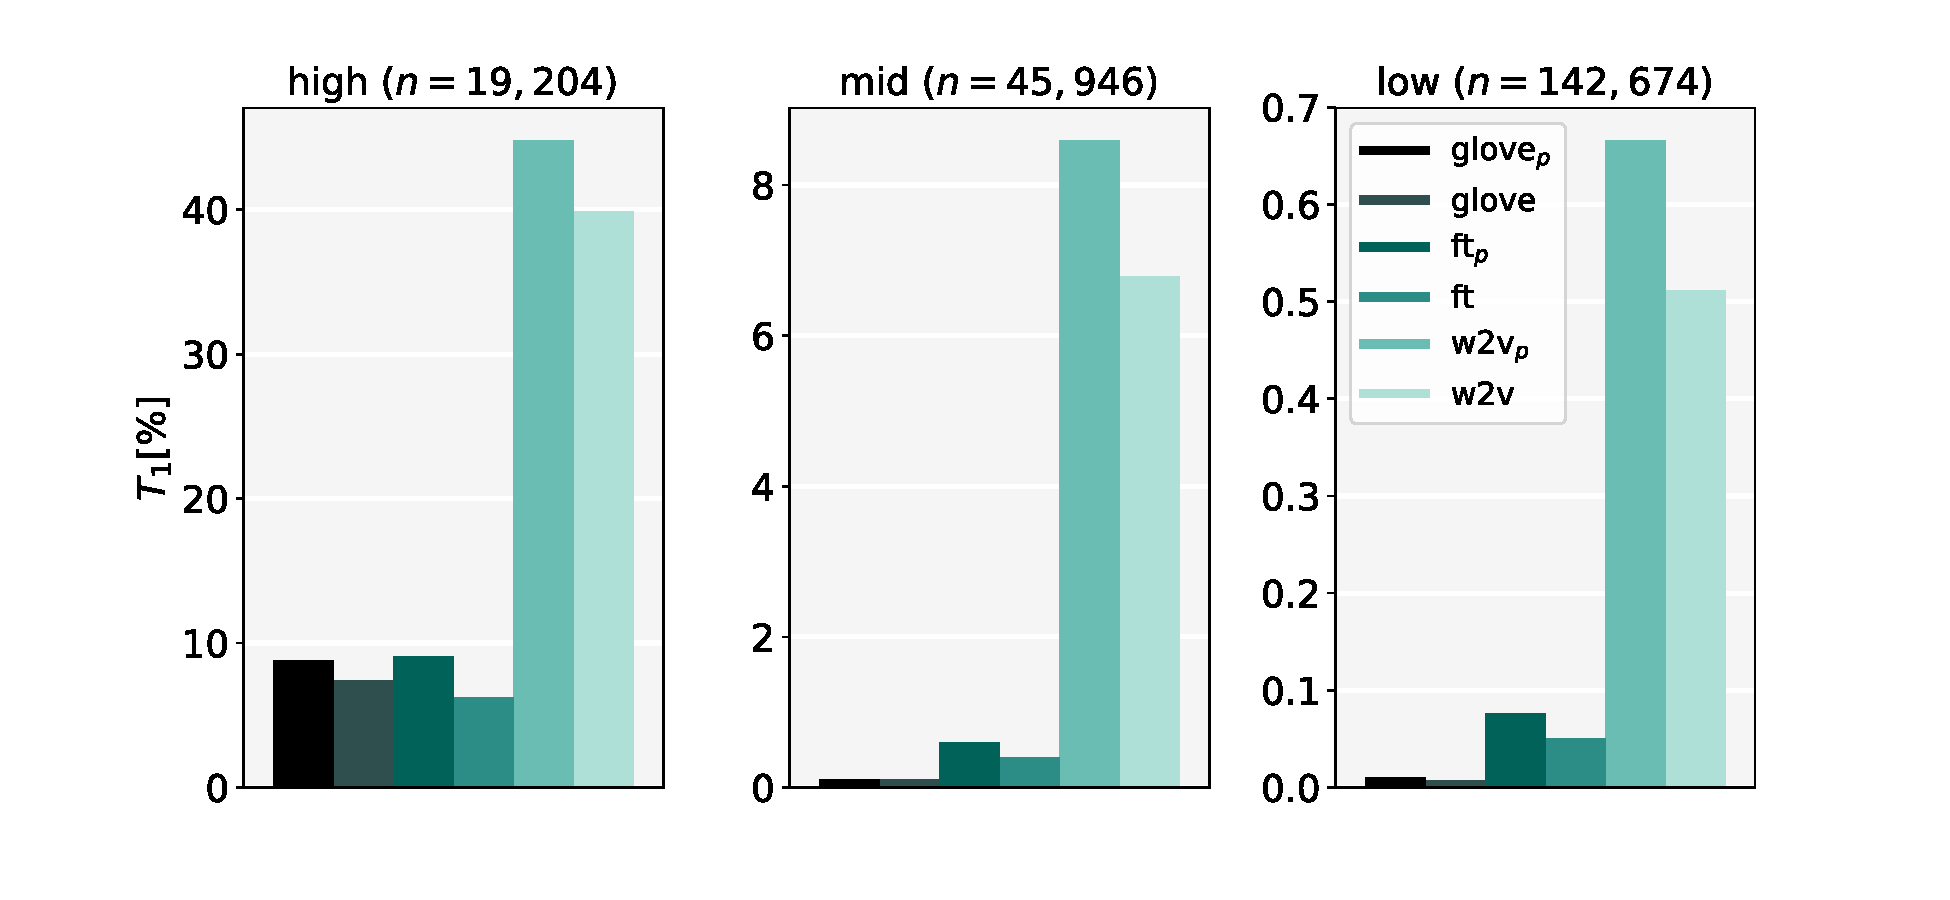
\includegraphics[width=0.47
    \textwidth]{fig/types_coverage_space_ny.pdf}
    %\vspace{-0.35in}
    \caption{NYT type coverage by training frequency and embedding space}
    %\vspace{-0.25in}
    \label{fig:type_coverage_space}
\end{figure}

\begin{figure}[h]
    \centering
    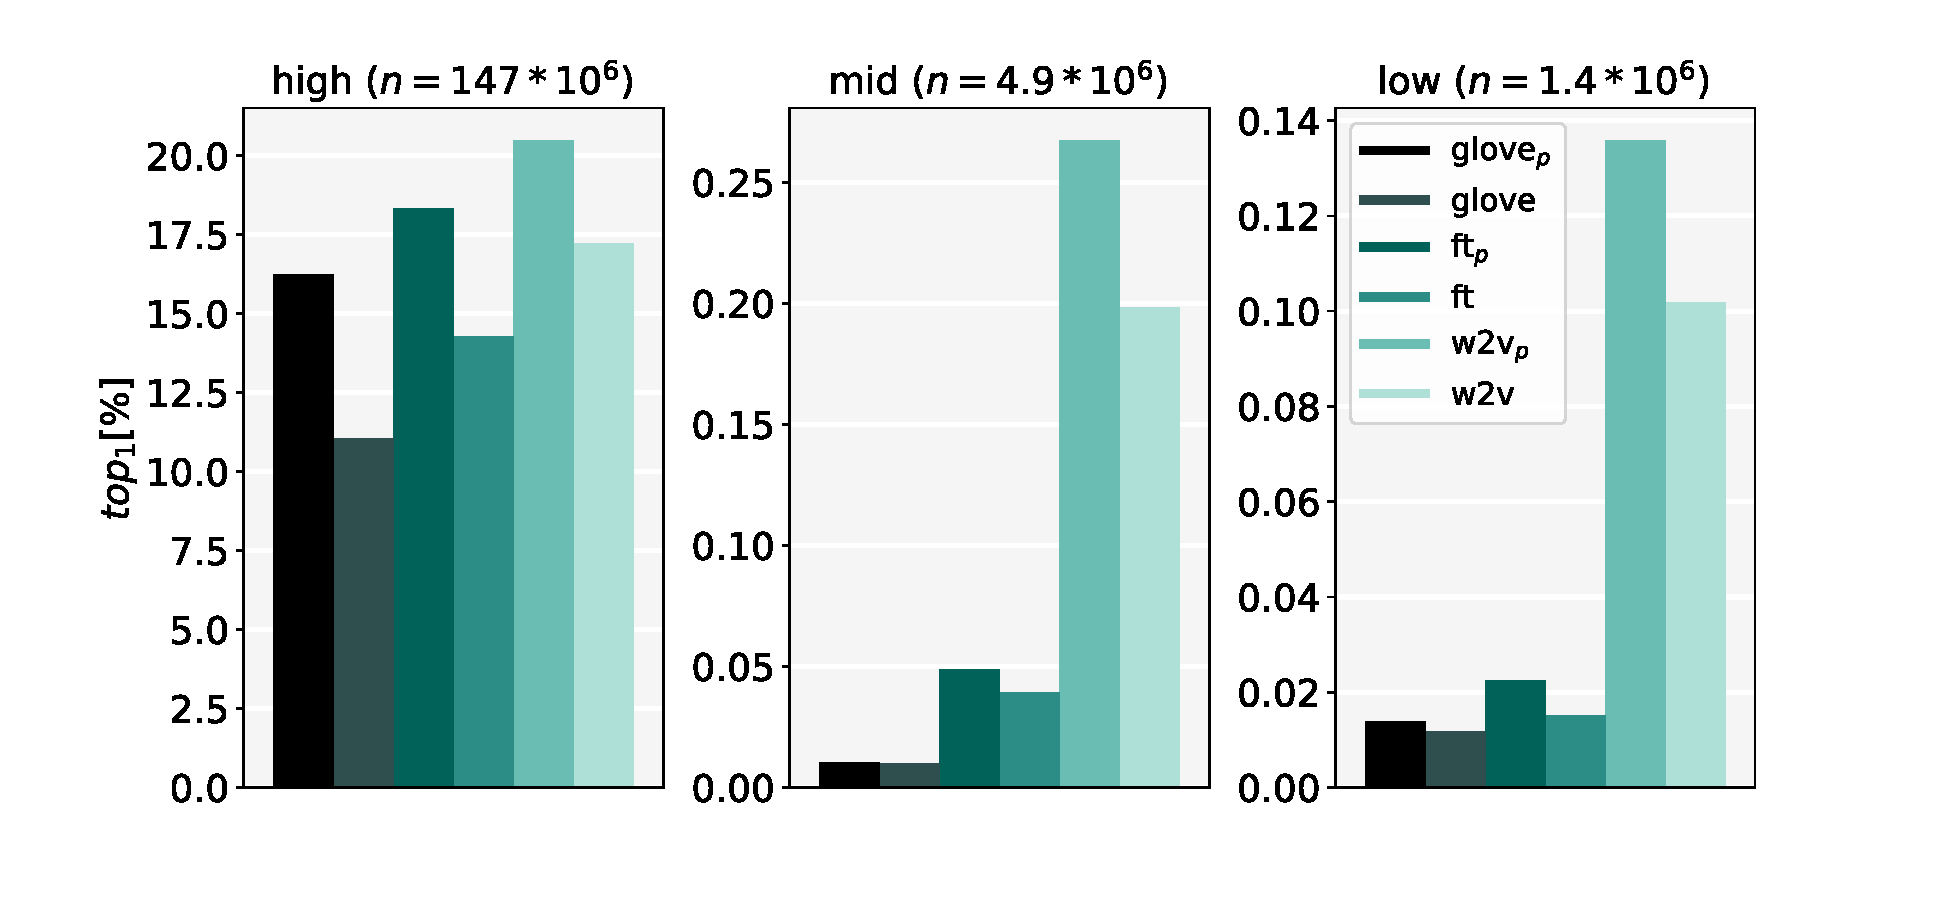
\includegraphics[width=0.47
    \textwidth]{fig/tokens_coverage_space_ny.pdf}
    %\vspace{-0.35in}
    \caption{NYT token hit rate by training frequency and embedding space}
    %\vspace{-0.25in}
    \label{fig:token_coverage_space}
\end{figure}

Another, more interesting reason may be due to the fact that fasttext does not directly generate the entire set of embedding words. Rather, it generates the most frequent ones, together with additional subwords made of pieces of less frequent words. 
Then, to represent the experiment's infrequent words in fasttext space it has to compose subwords together. 
A possible limitation is therefore the ability to capture the context of those rare words and represent them meaningfully in the space. 
A probable explanation for {\tt glv}'s lower performance was that we found it to create highly ``crowded'' regions, which in turn forced the model to learn to predict highly precisely the exact vector coordinates; as shown Table~\ref{space_50_p}, this proved difficult for the model to do.



%\section{Supplemental Material}
%\label{sec:supplemental}



\subsection{Qualitative Examples of NYT and PMC experiments}\label{qualit}

Table~\ref{tab:rare} provides actual examples taken from the test sets of both experiments (NYT as well as PMC) demonstrating the predictions of the continuous models vs. the categorical on less frequent word types.
As seen in Figures~\ref{fig:type_coverage_ny} and \ref{fig:token_coverage_ny}, as well as Figures~\ref{fig:type_coverage_pb} and \ref{fig:token_coverage_pb}, we observed no instances of a token being correctly predicted by the {\tt ctg} model in the lowest-frequency bin, and saw relatively few occurrences in the mid-frequency bin. 

In the examples below, the target token (that the model was required to predict) is in \textit{italics}. Where appropriate, we include a portion of the sentence following the target token, to provide the reader with context; recall that the model did not have access to this information at the time that it was queried.

\begin{table*}[t]
    \centering
\begin{tabularx}{\linewidth}{ll} 
\textbf{low bin} & \textbf{NYT predictions}  \\ 
    \addlinespace[1ex]

    {\tt G$_{p}$} & the 34th floor is still hushed a privileged cocoon of mahogany paneling brass wall \textit{sconces} \textcolor{gray}{...} \\
    {\tt ctg} & the 34th floor is still hushed a privileged cocoon of mahogany paneling brass wall \textit{street} \textcolor{gray}{...}\\
    \addlinespace[1ex]
    {\tt G} & \multirow{1}{*}{\parbox{13cm}{a report on japan trade was issued today by the labor-industry coalition on international trade a coalition that brings together the afl-cio and major u.s. steel textile and semiconductor workers along with the economic strategy institute an \textit{industry-financed} \textcolor{gray}{research group ...}}} \\ \\ \\
    \addlinespace[1ex]
     {\tt ctg} & \multirow{1}{*}{\parbox{13cm}{a report on japan trade was issued today by the labor-industry coalition on international trade a coalition that brings together the afl-cio and major u.s. steel textile and semiconductor workers along with the economic strategy institute an \textit{international} \textcolor{gray}{research group ...}}} \\ \\ \\
    \addlinespace[1ex]
\textbf{low bin} & \textbf{PMC predictions}  \\ 
    \addlinespace[1ex]
    {\tt G} & ... peptides were eluted by centrifugation followed by NUM additional \textit{elutions} \textcolor{gray}{with NUM $\mu$l} \\
    {\tt ctg} & ... peptides were eluted by centrifugation followed by NUM additional \textit{NUM} \textcolor{gray}{with NUM $\mu$l} \\
    \addlinespace[1ex]
    {\tt G$_{p}$} & ... are related to the constraint imposed on the electron \textit{wavefunctions} \textcolor{gray}{by the surface} \\
    {\tt ctg} & ... are related to the constraint imposed on the electron \textit{transport} \textcolor{gray}{by the surface} \\
    \addlinespace[1ex]
    {\tt G} &  ... owing to the anthropophilic and \textit{endophilic} \textcolor{gray}{behaviour of ...}\\
    {\tt ctg} & ... owing to the anthropophilic and \textit{unk} \textcolor{gray}{behaviour of ...}\\
    \addlinespace[1ex]
    {\tt G$_{p}$} & \multirow{1}{*}{\parbox{13cm}{the abnormal karyotypes from of cytogenetic studies include autosomal trisomies sex chromosome monosomy triploidy double \textit{trisomies} \textcolor{gray}{polyploidies ...}}}
     \\ \\
    \addlinespace[1ex]

    {\tt ctg} & \multirow{1}{*}{\parbox{13cm}{the abnormal karyotypes from of cytogenetic studies include autosomal trisomies sex chromosome monosomy triploidy double \textit{and} \textcolor{gray}{polyploidies ...}}} \\ \\
    \addlinespace[1ex]
    \textbf{mid bin} & \textbf{NYT predictions}  \\
    \addlinespace[1ex]
    {\tt G} & my piano teacher at the paris \textit{conservatory} \textcolor{gray}{a woman ...} \\
    {\tt ctg} & my piano teacher at the paris \textit{hotel} \textcolor{gray}{a woman ...} \\
    \addlinespace[1ex]

    {\tt G} & \multirow{1}{*}{\parbox{13cm}{among the NUM american women who have hysterectomies each year thousands may die prematurely of heart disease because doctors removed their \textit{ovaries} \textcolor{gray}{along with ...}}} \\ \\
    \addlinespace[1ex]
    {\tt ctg} & \multirow{1}{*}{\parbox{13cm}{among the NUM american women who have hysterectomies each year thousands may die prematurely of heart disease because doctors removed their \textit{way} \textcolor{gray}{along with ...}}} \\ \\
    \addlinespace[1ex]
    {\tt G} & \multirow{1}{*}{\parbox{13cm}{this mold covers the leaf in soot preventing the cells underneath from absorbing sunlight and conducting \textit{photosynthesis} \textcolor{gray}{eventually ...}}} \\ \\
    \addlinespace[1ex]
    {\tt ctg} & \multirow{1}{*}{\parbox{13cm}{this mold covers the leaf in soot preventing the cells underneath from absorbing sunlight and conducting \textit{the} \textcolor{gray}{eventually ...}}} \\ \\
    \addlinespace[1ex]
    \textbf{mid bin} & \textbf{PMC predictions}  \\
    \addlinespace[1ex]
    {\tt G} & this is further confirmed by detection of apoptotic and \textit{nonapoptotic} \textcolor{gray}{death ...} \\
    {\tt ctg} & this is further confirmed by detection of apoptotic and \textit{cell} \textcolor{gray}{death ...} \\
    \addlinespace[1ex] 
    {\tt G} & \multirow{1}{*}{\parbox{13cm}{in particular our objectives were to determine the association between NUM reported alcohol \textit{misuse} \textcolor{gray}{and hiv sexual ...}}} \\ \\
    \addlinespace[1ex] 
    {\tt ctg} & \multirow{1}{*}{\parbox{13cm}{in particular our objectives were to determine the association between NUM reported alcohol \textit{and} \textcolor{gray}{and hiv sexual ...}}} \\ \\ 
    \addlinespace[1ex] 
   {\tt G} & human infections are common following handling or processing of infected turkeys or \textit{ducks} \\
    {\tt ctg} & human infections are common following handling or processing of infected turkeys or \textit{by} \\
    \addlinespace[1ex] 
   {\tt G} & \multirow{1}{*}{\parbox{13cm}{NUM patients underwent cardiopulmonary resuscitation including NUM patients with respiratory arrest and pronounced \textit{bradycardia}}} \\ \\
    \addlinespace[1ex] 
   {\tt ctg} & \multirow{1}{*}{\parbox{13cm}{NUM patients underwent cardiopulmonary resuscitation including NUM patients with respiratory arrest and pronounced \textit{NUM}}} \\ \\
\end{tabularx}
  \caption{rare words' correct and incorrect predictions of continuous and categorical models respectively }
  \label{tab:rare}
\end{table*}

However, we provide here table~\ref{tab:catgeorical} as well which has the occurrences in which the categorical model predicted correctly while the continuous did not.

\begin{table*}[t]
    \centering
\begin{tabularx}{\linewidth}{ll} 
\textbf{mid bin} & \textbf{NYT predictions}  \\ 
    \addlinespace[1ex]
    {\tt ctg} & -lrb- eyman palm beach post -rrb- art includes a \textit{6-pica} \textcolor{gray}{color photo of book jacket}\\
    {\tt G} & -lrb- eyman palm beach post -rrb- art includes a \textit{compilation} \textcolor{gray}{color photo of book jacket}\\
    \addlinespace[1ex]
   {\tt ctg} & -lrb- this article is \textit{excerpted} \textcolor{gray}{from new scientist ...} \\
   {\tt G} & -lrb- this article is \textit{included} \textcolor{gray}{from new scientist ...} \\
    \addlinespace[1ex]
    {\tt ctg} & \multirow{1}{*}{\parbox{13cm}{the moscow military parade which has drawn no criticism across the russian political spectrum will put on display some of the very types of weapons that have been pounding chechnya since last december including t-72 tanks grad rocket-salvo \textit{launchers} \textcolor{gray}{and NUM ...}}} \\ \\ \\
    \addlinespace[1ex]
    {\tt G} & \multirow{1}{*}{\parbox{13cm}{the moscow military parade which has drawn no criticism across the russian political spectrum will put on display some of the very types of weapons that have been pounding chechnya since last december including t-72 tanks grad rocket-salvo \textit{helicopters} \textcolor{gray}{and NUM ...}}} \\ \\ \\
    \addlinespace[1ex]
    \textbf{mid bin} & \textbf{PMC predictions}  \\
    \addlinespace[1ex]
    {\tt ctg} & the sections were prepared by ultra microtone leica \textit{microsystems} \textcolor{gray}{and stained ...} \\
    {\tt G} & the sections were prepared by ultra microtone leica \textit{kontron} \textcolor{gray}{and stained ...} \\
    \addlinespace[1ex]
    {\tt ctg} & \multirow{1}{*}{\parbox{13cm}{height and weight was measured by trained technicians using standardized equipment with participants wearing light \textit{clothing} \textcolor{gray}{without shoes}}} \\ \\
    \addlinespace[1ex]
    {\tt G} & \multirow{1}{*}{\parbox{13cm}{height and weight was measured by trained technicians using standardized equipment with participants wearing light \textit{shoes} \textcolor{gray}{without shoes}}} \\ \\
    \addlinespace[1ex]
    {\tt ctg} & \multirow{1}{*}{\parbox{13cm}{this gave recommended retail prices rrp for all major cigarette brands for the uk market ie great \textit{britain} \textcolor{gray}{and northern ireland}}} \\ \\
    \addlinespace[1ex]
    {\tt G} & \multirow{1}{*}{\parbox{13cm}{this gave recommended retail prices rrp for all major cigarette brands for the uk market ie great \textit{livelihood} \textcolor{gray}{and northern ireland}}} \\ \\
\end{tabularx}
  \caption{mid bin correct and incorrect predictions of categorical and continuous models respectively}
  \label{tab:catgeorical}
\end{table*}

%correct categorical NYT:

% \begin{itemize}
%   \item {\tt ctg}: -lrb- eyman palm beach post -rrb- art includes a \textit{6-pica} color photo of book jacket
%   \item {\tt ctg}: -lrb- eyman palm beach post -rrb- art includes a \textit{compilation} color photo of book jacket
%   \item {\tt ctg}: -lrb- this article is \textit{excerpted} from new scientist a weekly science and technology magazine based in london
%   \item {\tt G}: -lrb- this article is \textit{included} from new scientist a weekly science and technology magazine based in london
%   \item {\tt ctg}: the moscow military parade which has drawn no criticism across the russian political spectrum will put on display some of the very types of weapons that have been pounding chechnya since last december including t-72 tanks grad rocket-salvo \textit{launchers} and NUM fighter-bombers
%   \item {\tt G}: the moscow military parade which has drawn no criticism across the russian political spectrum will put on display some of the very types of weapons that have been pounding chechnya since last december including t-72 tanks grad rocket-salvo \textit{helicopters} and NUM fighter-bombers
% \end{itemize}

%correct categorical PB:

% \begin{itemize}
%   \item {\tt ctg}: the sections were prepared by ultra microtone leica \textit{microsystems} and stained with uranyl acetate and citrate
%   \item {\tt G}: the sections were prepared by ultra microtone leica \textit{kontron} and stained with uranyl acetate and citrate
%   \item {\tt ctg}: height and weight was measured by trained technicians using standardized equipment with participants wearing light \textit{clothing} without shoes and bmi was calculated
%   \item {\tt G}: height and weight was measured by trained technicians using standardized equipment with participants wearing light \textit{shoes} without shoes and bmi was calculated
%   \item {\tt ctg}: this gave recommended retail prices rrp for all major cigarette brands for the uk market ie great \textit{britain} and northern ireland wherein northern ireland accounts for just NUM \% of total volume
%   \item {\tt G}: this gave recommended retail prices rrp for all major cigarette brands for the uk market ie great \textit{livelihood} and northern ireland wherein northern ireland accounts for just NUM \% of total volume
  
% \end{itemize}

% \begin{itemize}
%   \item {\tt G$_{p}$}: the 34th floor is still hushed a privileged cocoon of mahogany paneling brass wall \textit{sconces} a meeting table longer than a limousine carpeting the color of money and a men 's room paneled in marble and granite
%   \item {\tt ctg}: the 34th floor is still hushed a privileged cocoon of mahogany paneling brass wall \textit{street} a meeting table longer than a limousine carpeting the color of money and a men 's room paneled in marble and granite
%   \item {\tt G}: a report on japan trade was issued today by the labor-industry coalition on international trade a coalition that brings together the afl-cio and major u.s. steel textile and semiconductor workers along with the economic strategy institute an \textit{industry-financed} research group that advocates more open markets with tokyo
%   \item {\tt ctg}: a report on japan trade was issued today by the labor-industry coalition on international trade a coalition that brings together the afl-cio and major u.s. steel textile and semiconductor workers along with the economic strategy institute an \textit{international} research group that advocates more open markets with tokyo
%   \item {\tt G$_{p}$}: dos \textit{semanas} antes de las elecciones el rival saco de la manga a una ex novia de lula con la cual este habia tenido una hija de cuya manutencion dijo la mujer jamas se habia ocupado
%   \item {\tt ctg}: dos \textit{is} antes de las elecciones el rival saco de la manga a una ex novia de lula con la cual este habia tenido una hija de cuya manutencion dijo la mujer jamas se habia ocupado
% \end{itemize} 

% \begin{itemize}
%   \item {\tt G}: the resulting digested peptides were eluted by centrifugation followed by NUM additional \textit{elutions} with NUM $\mu$l
%   \item {\tt ctg}: the resulting digested peptides were eluted by centrifugation followed by NUM additional \textit{NUM} with NUM $\mu$l
%   \item {\tt G$_{p}$}: these particles are commonly known as quantum dots because the sizedependent changes in electronic structure are related to the constraint imposed on the electron \textit{wavefunctions} by the surface
%   \item {\tt ctg}: these particles are commonly known as quantum dots because the sizedependent changes in electronic structure are related to the constraint imposed on the electron \textit{transport} by the surface
%   \item {\tt G$_{p}$}: the abnormal karyotypes from of cytogenetic studies include autosomal trisomies sex chromosome monosomy triploidy double \textit{trisomies} polyploidies as well as structural rearrangements
%   \item {\tt ctg}: the abnormal karyotypes from of cytogenetic studies include autosomal trisomies sex chromosome monosomy triploidy double \textit{and} polyploidies as well as structural rearrangements
%   \item {\tt G}: the gel patterns were scanned using an arcus \textit{agfa} scanner and analyzed using the image analysis nih software
%   \item {\tt ctg}: the gel patterns were scanned using an arcus \textit{software} scanner and analyzed using the image analysis nih software
%   \item {\tt G}: owing to the anthropophilic and \textit{endophilic} behaviour of the vectors they need to enter houses to get their blood meals from humans
%   \item {\tt ctg}: owing to the anthropophilic and \textit{UNK} behaviour of the vectors they need to enter houses to get their blood meals from humans
% \end{itemize} 

% \subsubsection{mid frequency bin}

% NYT
% \begin{itemize}
%   \item {\tt G}: among the NUM american women who have hysterectomies each year thousands may die prematurely of heart disease because doctors removed their \textit{ovaries} along with their wombs a new study suggests
%   \item {\tt ctg}: among the NUM american women who have hysterectomies each year thousands may die prematurely of heart disease because doctors removed their \textit{way} along with their wombs a new study suggests
%   \item {\tt G}: this mold covers the leaf in soot preventing the cells underneath from absorbing sunlight and conducting \textit{photosynthesis} eventually killing the leaf
%   \item {\tt ctg}: this mold covers the leaf in soot preventing the cells underneath from absorbing sunlight and conducting \textit{the} eventually killing the leaf
%   \item {\tt G}: my piano teacher at the paris \textit{conservatory} %a woman of astonishing technique minimal teaching skill and sublime ignorance of any style but her own had once over a period of <number> or <number> lessons played the keyboard pieces of ravel for the composer
%   \item {\tt ctg}: my piano teacher at the paris \textit{hotel}
% \end{itemize} 

% PB
% \begin{itemize}
%   \item {\tt G}: this is further confirmed by detection of apoptotic and \textit{nonapoptotic} death in a5 and e9 cells following transfection of synthetic ncrrnas consistent with a recent report using human cells
%   \item {\tt ctg}: this is further confirmed by detection of apoptotic and \textit{cell} death in a5 and e9 cells following transfection of synthetic ncrrnas consistent with a recent report using human cells 
%   \item {\tt G}: in particular our objectives were to determine the association between NUM reported alcohol \textit{misuse} and hiv sexual risk behaviors NUM reported alcohol misuse and hiv screening uptake and NUM reported sexual risk and hiv screening uptake in the absence of any interventions
%   \item {\tt ctg}: in particular our objectives were to determine the association between NUM reported alcohol \textit{and} and hiv sexual risk behaviors NUM reported alcohol misuse and hiv screening uptake and NUM reported sexual risk and hiv screening uptake in the absence of any interventions
%   \item {\tt G}: human infections are common following handling or processing of infected turkeys or \textit{ducks}
%   \item {\tt ctg}: human infections are common following handling or processing of infected turkeys or \textit{by}
%   \item {\tt G}: NUM patients underwent cardiopulmonary resuscitation including NUM patients with respiratory arrest and pronounced \textit{bradycardia}
%   \item {\tt ctg}: NUM patients underwent cardiopulmonary resuscitation including NUM patients with respiratory arrest and pronounced \textit{NUM}
%   \item {\tt G}: by the time he turned NUM in NUM he had been arrested a dozen times for civil \textit{disobedience} %but he did not stop then in NUM he and other protesters were arrested and charged with trespassing after they demonstrated at cape canaveral air force station against th test launching of a trident NUM missile
%   \item {\tt ctg}: by the time he turned NUM in NUM he had been arrested a dozen times for civil \textit{war}
% \end{itemize} 





% \begin{table}[h]
% \begin{center}
% \begin{tabular}{lrrr}
% space &  $top_{1}(top_{10})$ & $T_{1}(T_{10})$ & $M$\\ \hline
% w2v & $16.46(27.45)$ & $11,534(27,921)$ & $0.20$   \\
% w2v$_{p}$ & $19.56(30.30)$ & $13,540(32,140)$ & $0.23$  \\
% ft & $10.67(18.66)$ & $875(2,584)$ & $0.13$ \\
% ft$_{p}$ & $15.06(23.40)$ & $1,111(3,211)$ & $0.18$\\
% glove & $10.36(19.19)$ & $1,007(2,253)$ & $0.13$    \\
% glove$_{p}$ & $16.86(29.74)$ & $1,221(2,666)$ & $0.21$ \\\\
% \end{tabular}
% \end{center}
% \vspace{-0.1in}
% \caption{\label{space_50_g}{NYT embedding spaces effect on {\tt G$_{50}$}}}
% \end{table}


% \begin{table}[h]
% \begin{center}
% \begin{tabular}{lrrr}
% space &  $top_{1}(top_{10})$ & $T_{1}(T_{10})$ & $M$\\ \hline
% w2v & $18.15(29.15)$ &  $6,194(17,905)$ & $0.22$    \\
% w2v$_{p}$ & $20.91(31.06)$ & $7,659(21,221)$ & $0.24$  \\
% ft & $11.96(16.89)$ & $208(664)$ & $0.13$ \\
% ft$_{p}$ & $14.46(19.83)$ & $338(985)$ & $0.16$  \\
% glove & $12.34(17.29)$ & $399(987)$ & $0.14$  \\
% glove$_{p}$ & $15.21(24.91)$ & $536(1,259)$ & $0.18$ \\
% \end{tabular}
% \end{center}
% \vspace{-0.1in}
% \caption{\label{space_200_g}{NYT embedding spaces effect on {\tt G$_{200}$}}}
% \end{table}

%\subsection{Feature-Based Decoding contin.}\label{decoding_cont}

%Our intent is that if adding this information is fruitful, a future step is to investigate how to incorporate this knowledge into the system. One possible way is to train a small-footprint POS model (softmax-based) for the decoding step (separated from the main model), that provides an oracle about the expected POS of the target term that is being searched, which will provide a refined list of candidates. Since our mechanism as well as the model we intend to build is separated, it has the advantage of applying it post-hoc, and is independent w.r.t. the training of the model. We note that in order to decode with POS, one has to have access to such data. Currently to implement this decoding we provided the expected true POS of the target data, and for every candidate we search its associated POS from a dict formed on the training set. This experiment contained $1,470,744$ and $67,044$ tokens and types respectively. 
%Figure~\ref{fig:pos_analysis} shows the improvement for small scale experiment conducted on NYT dataset, though the results improve for every experiment we ran. 

% \begin{figure}[h]
%     \centering
%     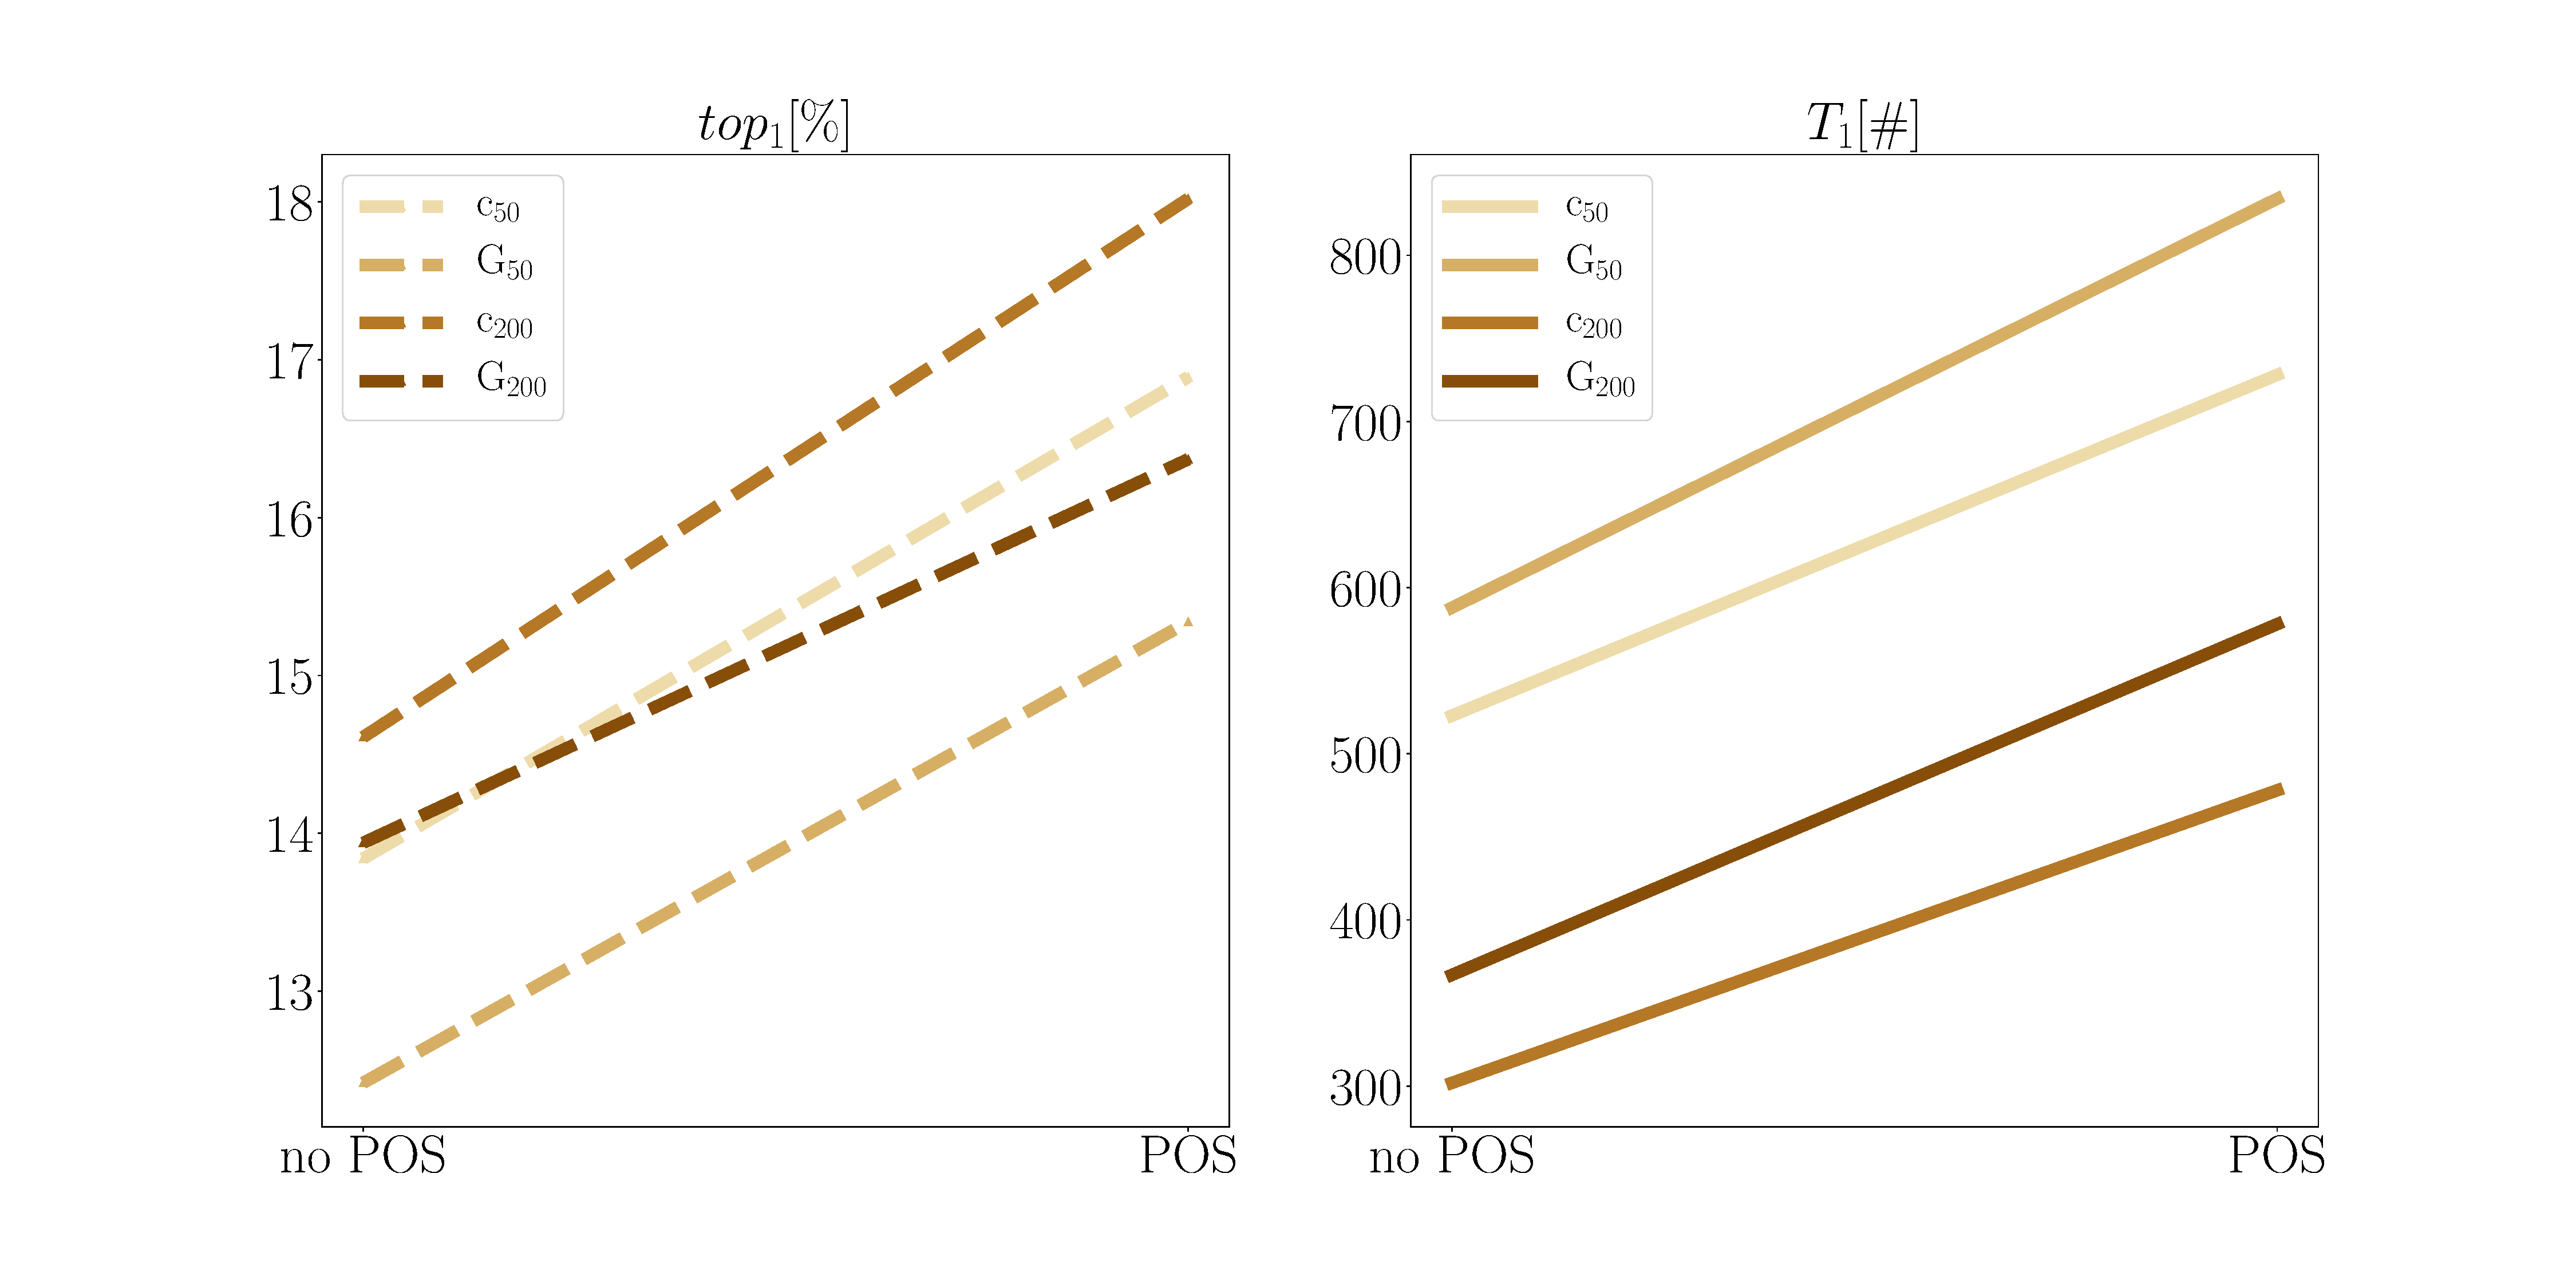
\includegraphics[width=0.47
%     \textwidth]{fig/pos_delta.pdf}
%     %\vspace{-0.35in}
%     \caption{feature decoding with POS employed to small scale NYT model}
%     %\vspace{-0.25in}
%     \label{fig:pos_analysis}
% \end{figure}

\end{document}
